
\PassOptionsToPackage{table,xcdraw}{xcolor}
\documentclass[sigconf]{acmart}

\copyrightyear{2026}
\acmYear{2026}
\setcopyright{cc}
\setcctype{by}
\acmConference[CF Companion '26 ]{Proceedings of the 23rd ACM International Conference on Computing Frontiers}{May 19--21, 2026}{Catania, Italy}
\acmBooktitle{Proceedings of the 23rd ACM International Conference on Computing Frontiers (CF Companion '26 ), May 19--21, 2026, Catania, Italy}
\acmDOI{10.1145/3801488.3807896}
\acmISBN{979-8-4007-2569-2/2026/05}

\usepackage[T1]{fontenc}
\usepackage{booktabs}
\usepackage{multirow}
\usepackage{array}
\usepackage{amsmath,amsfonts}
\usepackage{algorithmic}
\usepackage{graphicx}
\usepackage{textcomp}
\usepackage{bbding}
\usepackage{pifont}
\usepackage{tikz}
\usetikzlibrary{shapes.geometric,arrows,positioning,fit}
\usepackage{rotating}
\usepackage{enumitem}
%\usepackage{siunitx}
\definecolor{LightGray}{gray}{0.9}
\newcolumntype{C}[1]{>{\centering\arraybackslash}p{#1}}
\newcommand{\methodname}{ASSESS}
\newcommand{\methoddis}{Analysis of Side-channel Security through Enhanced pre-Silicon Simulations}
\newif\ifblind
\blindfalse

\setlength{\abovecaptionskip}{4pt}
\setlength{\belowcaptionskip}{-2pt}
\begin{document}
\title{Systematic Comparison and Improvement of Pre-silicon Leakage Analysis Tools}
\author{Abolfazl Sajadi}
%\orcid{0000-0003-0657-7022}
\affiliation{%
  \institution{LIACS, Leiden University}
  \city{Leiden}
  \country{The Netherlands}
}
\email{a.sajadi@liacs.leidenuniv.nl}

\author{Nusa Zidaric}
%\orcid{0000-0001-9308-7392}
\affiliation{%
  \institution{LIACS, Leiden University}
  \city{Leiden}
  \country{The Netherlands}
}
\email{n.zidaric@liacs.leidenuniv.nl}

\author{Todor Stefanov}
%\orcid{0000-0001-6006-9366}
\affiliation{%
  \institution{LIACS, Leiden University}
  \city{Leiden}
  \country{The Netherlands}
}
\email{t.p.stefanov@liacs.leidenuniv.nl}

\author{Nele Mentens}
%\orcid{0000-0001-8753-7895}
\affiliation{%
  \institution{LIACS,Leiden University}
  \city{Leiden}
  \country{The Netherlands}
}
\affiliation{%
    \institution{COSIC, ES\&S, KU Leuven}
  \city{Leuven}
  \country{Belgium}
}
\email{n.mentens@liacs.leidenuniv.nl}
\begin{abstract}

{Side-channel attacks exploit physical information leakage, such as power consumption, to recover secret data, posing a serious threat to hardware security. To address these concerns early in the design cycle, pre-silicon leakage analysis is becoming a fundamental and mandatory step when building secure hardware. 

The first part of this paper focuses on the systematic comparison of three notable pre-silicon side-channel leakage evaluation methodologies: RTL-PAT, PATCH, and ACA. The comparison is two-fold: (1) A qualitative comparison, based on a systemization of knowledge that decomposes the existing methodologies into three phases; (2) A quantitative comparison, focusing on the following metrics: runtime, and leakage localization granularity. For fairness, we run all experiments under identical conditions on a common benchmark: a 32-bit RISC-V core %(Ibex) 
running a software implementation of Tiny-AES, %(Tiny-AES), 
and a hardware AES coprocessor, synthesized using a 22nm standard-cell library. The systematic comparison allows us to highlight the trade-offs between module-level vs. gate-level detection, i.e., coarse-grained vs. fine-grained leakage localization, and to identify tool-induced runtime overheads.
 
Based on these findings, the second part of this paper proposes an improved ACA-inspired methodology: \methodname\ (\methoddis). It leverages a cycle-accurate toggle activity correlation, while bypassing the expensive time-based power extraction. The experimental results demonstrate that our approach preserves the fine-grained leakage localization of ACA while significantly reducing the analysis time. % and memory usage. 
Our open-source methodology enables frequent leakage evaluations during the iterative ASIC design process. It empowers designers to pinpoint the leakage and apply targeted countermeasures before tape-out, reducing fabrication costs and strengthening hardware security.}
\end{abstract}
\keywords{Side-Channel Leakage, Netlist Analysis, Power SCA, RISC-V, AES}%Tiny-AES \and Ibex.}
\maketitle
\section{Introduction}
{
Digital hardware is the core of all modern technologies, ranging from cloud data centers to medical devices. Exploitable information leakage through side-channels has devastating consequences, such as privacy loss or even critical infrastructure failure. \emph{Side-Channel Analysis} (SCA) can recover secrets, e.g., encryption keys, by observing physical artifacts such as power consumption, electromagnetic radiation, or execution time, rather than by breaking the underlying mathematics. Well-known power-analysis attacks on smart-card implementations of AES~\cite{cardpo,10752477,kocher} and on standardized Trusted Platform Module (TPM) 2.0 security chips~\cite{tpm} extracted the keys in minutes, even when the cryptographic algorithms themselves were secure. Such incidents underscore the need to identify and mitigate side-channel vulnerabilities before chips are deployed. Nevertheless, the iterative process of analyzing chips after fabrication, and re-designing and re-fabricating them when side-channel weaknesses are detected, adds months and significant cost to the schedule, and fabricating an ASIC test chip solely for power analysis is rarely feasible. Therefore, there is a need to discover and neutralize leakage during the hardware design cycle (pre-silicon), not after fabrication (post-silicon).
While post-silicon evaluation remains a final safeguard, it is reactive and expensive.
Pre-silicon leakage detection enables engineers to insert targeted countermeasures, iterate quickly, and meet their goals while avoiding the need for broad, high-overhead countermeasures.
However, pre-silicon leakage detection analysis has to overcome several challenges: (i) Adequate leakage localization granularity is needed to pinpoint which nets or gates leak, such that countermeasures remain local and low-overhead;  
(ii) The analysis must correlate closely with real silicon behavior, otherwise some leakage sources may not be discovered; (iii) Given the iterative nature of ASIC design, each leakage detection analysis must be computationally efficient to support frequent design re-evaluation after design refinements and back-end adjustments.


Several existing ASIC-aware pre-silicon evaluation methodologies have already tried to address these challenges. 
Notable examples are RTL-PAT~\cite{RTL_PSC}, which focuses on module-level leakage evaluation, and PATCH~\cite{PATCH} and ACA~\cite{ACA}, which focus on gate-level leakage evaluation. However, to the best of our knowledge, no prior work has performed a unified quantitative comparison of these methodologies using the same technology node and benchmarks. Consequently, the community lacks a clear understanding of the precise trade-offs not just qualitatively, but quantitatively between module-level and gate-level approaches. 
In addition, the existing methodologies have important limitations, i.e., RTL-PAT lacks fine-grained leakage localization, while PATCH and ACA incur prohibitive computational costs due to the reliance on expensive time-series power extraction. 

Therefore, in this paper, we provide a unified quantitative comparison of these methodologies and propose an improved methodology for pre-silicon \emph{Power Side-Channel} (PSC) leakage evaluation that addresses the aforementioned limitation by  combining gate-level precision with the speed required to enable efficient iterative ASIC design. More specifically, the novel contributions of this paper can be summarized as follows:

\noindent 
1. We provide a \textbf{systemization of knowledge} by decomposing the {RTL-PAT}, {PATCH}, and {ACA} methodologies into distinct phases, namely Simulation, Power Estimation, and Leakage Assessment. This allows us to present a fair quantitative comparison under identical conditions, i.e., the same experimental setup, ASIC technology node (\mbox{GF\textsuperscript{\textregistered}
22FDX}), and benchmark design (RISC-V/Ibex).

  %\item 
\noindent 
2. We develop a \textbf{common evaluation framework} by implementing and documenting practical refinements that improve the accuracy and/or runtime of each methodology. By making our framework and benchmarks available as open-source, we enable the research community to reuse this framework for future optimizations and evaluations.

\noindent 
3. Based on critical bottlenecks, identified during the aforementioned quantitative comparison, we design and implement a new open-source methodology called \textbf{\methodname{}} (\methoddis). \methodname{} is a cycle-accurate methodology that supports gate-level leakage localization, hence addressing challenge (i). To address challenge (ii), our methodology requires one run with a commercial power estimation tool using a targeted ASIC standard-cell library. addressing challenge (iii), ASSESS eliminates the expensive time-series power extraction by cycle-accurate analysis of the nets' switching activity within the  design.
%\end{enumerate}








This paper is organized as follows. Section~\ref{sec:related} briefly reviews related work. Section~\ref{sec:Comparative} presents an overview of the three previously proposed methodologies selected for comparison. Section~\ref{sec:comparison} compares these methodologies and experimental results, and offers improvement suggestions. Section~\ref{sec:Methodology} details our proposed methodology and examines its outcomes. Finally, Section~\ref{sec:Conclusions} concludes the paper.

}

\section{Related Work}
\label{sec:related}


Side-channel vulnerabilities can be detected at any design level of abstraction, from detailed transistor-level simulations to higher-level gate and RTL analyses where the choice of abstraction level strongly affects both the detection accuracy and runtime. At the transistor level, some authors rely on circuit simulation with SPICE to estimate the power consumption and identify potential sources of leakage~\cite{SpiceLV}. Although this approach offers high accuracy, it also requires considerable computational resources and scales poorly for larger designs.




 
Saidoyoki \emph{et al.}~\cite{Saidoyoki} introduces a dual-setting evaluation platform that compares pre-silicon leakage estimations with post-silicon measurements, demonstrating that early-stage simulations can achieve fine-grained localization resolution and robust root-cause analysis. Their work highlights the necessity of leakage analysis at multiple levels of abstraction (from RTL to layout).




Still at the RTL level, PSC-TG~\cite{PSC-TG} uses test-pattern generation and information flow tracking to detect worst-case power side-channel leakage before fabrication. By identifying sensitive variables and generating inputs that maximize leakage, PSC-TG allows early, cost-effective countermeasures without requiring an actual silicon prototype. The successor of PSC-TG, RTL‑PAT (formerly RTL‑PSC)~\cite{RTL_PSC}, also performs a side‑channel leakage assessment at the RTL stage, offering a comparatively fast and technology‑agnostic solution. Its emphasis on module‑level analysis nevertheless overlooks finer‑grained factors such as glitches, which are known sources of side‑channel leakage~\cite{glitches}, and disregards placement and routing details. Designers therefore cannot always determine which specific nets or signals dominate the leakage, limiting the accuracy of any subsequent countermeasures.
SCAR~\cite{scar} applies a graph neural network to RTL control–data flow graphs to flag ``leaky'' code and then uses large language models (LLM) to auto-patch the code. Their approach depends on manually labeled ``leaky'' modules and does not capture post-routing effects (e.g., glitches and coupling). The scalability %and verification 
of LLM-generated mitigations remains an open challenge.

Moving further down in the design flow abstraction levels, several methodologies operate directly on gate‑level netlists. PATCH \cite{PATCH} ranks nets by correlating each net’s toggling activity with the instantaneous total power trace. Since the analysis is restricted to pre‑selected \emph{sensitive windows}, glitch‑induced leakage outside those windows can remain undetected. Architecture Correlation Analysis (ACA)~\cite{ACA} achieves even finer localization granularity by correlating the simulated power of every gate with a hypothesized leakage model. Yao \emph{et al.}~\cite{GateLevelACA} applied ACA to both a stand‑alone AES coprocessor and a RISC‑V SoC, showing that only a few percent of gates account for the bulk of the observable leakage. The gate‑level visibility comes at a cost: extracting and analyzing thousands of time-series power traces required by ACA dominates the simulation runtime on SoC‑scale designs. In general, both PATCH and ACA depend on accurate time-series of power data from commercial EDA tools, which become increasingly expensive (in time and effort) to generate when the design size and process complexity increase. PathFinder~\cite{PATHFINDER} builds on ACA by using ACA-based localization to select high-leakage logic cones (i.e., gate-level region spanning from primary inputs to primary outputs) before inserting logic-level obfuscations, so any speed or accuracy improvements to ACA directly benefit PathFinder. Since our flow also builds on ACA, our results will also improve PathFinder.
Bhasin et al.~\cite{Bhasin} generate design-time SCA traces via SPICE/FAST-SPICE or timing-annotated VCD (Value Change Dump) with equal-weight transitions. However, they do not provide per-gate Leakage Impact Factors (LIFs), so the approach lacks gate-level leakage localization. Unlike Count Your Toggles~\cite{CountYourToggles}, which focuses on leakage estimation using aggregate switching activity, our methodology performs cycle-accurate, gate-level leakage localization with per-gate LIF ranking while remaining technology-aware.

Another line of work operates at the post-placement stage. Karna \cite{Karna} adjusts the power profile by swapping gates. This can reduce leakage when sufficient positive timing slack is available, but that requirement restricts design flexibility and does not directly reveal which nets are the most leakage-prone. 

Our goal differs: we target gate-level, technology-aware, label-free leakage localization with per-gate LIFs and reproducible timing. Hence, we do not adopt SCAR’s ML/auto-patch flow. Instead, our method quantifies leakage on the ASIC fabric that will actually be fabricated rather than proposing edits at RTL. The remainder of this paper focuses on the reconstruction, comparison and improvement of three notable pre-silicon PSC leakage assessment methodologies, that operate on different levels of abstraction, from RTL down to placed gate-level netlists, namely RTL‑PAT, PATCH, and ACA. 

\section{RTL-PAT, PATCH and ACA in Three Phases}
\label{sec:Comparative}

In this section, we examine the three main phases common to all three methodologies, namely simulation, power estimation, and leakage assessment, shown at the top part of Fig.~\ref{fig:method}, \ref{fig:patch} and \ref{fig:ACA}. This decomposition was already used by the authors of the RTL-PAT methodology~\cite{RTL_PSC}, and we apply it to all methodologies examined in this paper. We represent the three existing methodologies graphically for easier comprehension of subtle differences. The comparison in this section focuses on the utilized leakage models and the leakage localization granularity the methodologies can achieve.  Whenever a methodology requires time-series power traces, we assume that these traces are obtained by using a \emph{commercial power tool (CPT)} e.g., Synopsys PrimeTime~PX or Cadence\textsuperscript{\tiny\textregistered} Joules.

 







\subsection{RTL‑PAT: PSC Leakage Assessment at RTL}
RTL‑PAT~\cite{RTL_PSC} is a pre-silicon SCA methodology that operates directly at the RTL design. It statistically analyzes differences in module-level switching activities, enabling designers to efficiently identify leakage-prone modules in the design. Fig.~\ref{fig:method} outlines the main phases of RTL-PAT.

\label{sec:RTL‑PAT}
 \begin{figure}[!t]
     \centering
     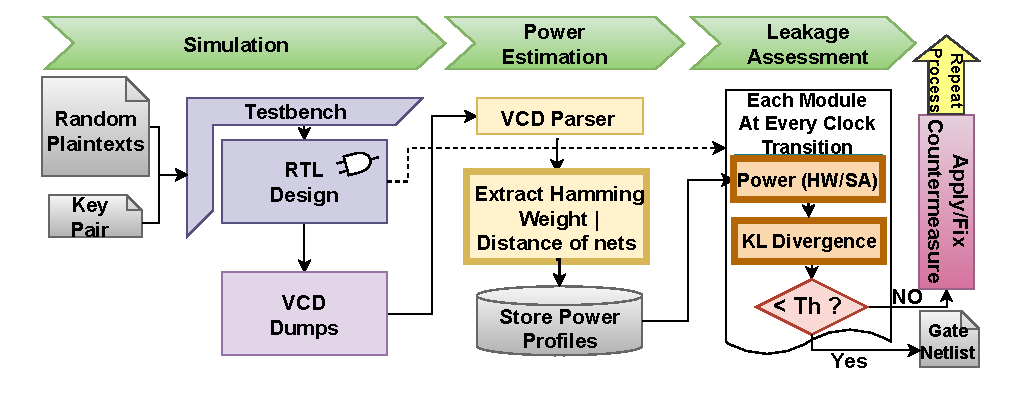
\includegraphics[width=0.5\textwidth]{Pictures/RTL_PSCbold.pdf}
     \caption{The RTL-PAT methodology, based on Fig.\,1 in~\cite{RTL_PSC}.}
     \label{fig:method}
     \vspace{-2mm}
 \end{figure}




\noindent{\bf Simulation. }
A common SCA practice %in AES leakage assessment 
is to select two keys with the maximum Hamming distance (HD) (typically 0x00$\dots$00 and 0xFF$\dots$FF) to maximize the statistical separation between the resulting power distributions. This choice is made under the assumption that the plaintext is XORed with the key, and two keys with a larger Hamming distance are likely to produce more distinct switching activities. RTL simulations are executed separately for each key using the same set of $N$ random plaintexts, and the signal transitions are recorded into VCD files that capture the switching activities.

\noindent{\bf Power Estimation. }
The generated VCD files in the first step are parsed to estimate dynamic power consumption using two common models. The first model, Hamming Weight (HW), estimates the power consumption as proportional to the number of nets at logic '1', based on a simplified CMOS characteristic where storing or driving a logic ‘1’ is assumed to incur higher power than a logic ‘0’. The second model, 
 HD,  estimates the power consumption as proportional to the number of net transitions, either from '0' $\to$ '1' or '1' $\to$ '0', based on the assumption that the transitions cause dynamic power consumption.

\noindent{\bf Leakage Assessment. }
To assess how easily an attacker could distinguish two secret keys, RTL‑PAT compares the simulated power‑consumption distributions produced by each key.  
The chosen statistical estimator for this comparison is the \emph{Kullback–Leibler} divergence ($D_{KL}$). The larger \(D_{\mathrm{KL}}\) is, the more distinguishable the two keys are and 
the more vulnerable the design becomes. Assuming the two distributions \(X\) and \(Y\) are Gaussian with means
\(\mu_X, \mu_Y\) and variances \(\sigma_X^{2},\sigma_Y^{2}\), the closed‑form $D_{KL}$
expression is given as: %in Eq.~\ref{eq:KLdivergence}.

\begin{equation}
D_{\mathrm{KL}}\!\bigl(X\parallel Y\bigr)=
\frac{(\mu_X-\mu_Y)^{2}+\sigma_X^{2}-\sigma_Y^{2}}{2\sigma_Y^{2}}
\;+\;
\ln\!\Bigl(\tfrac{\sigma_Y}{\sigma_X}\Bigr)
\label{eq:KLdivergence}
\end{equation}

RTL‑PAT flags every module whose $D_{KL}$ score exceeds a user selected
threshold.  The original work tabulates thresholds in terms of an
\emph{adversary failure probability} \(P_r\) (Table~\ref{tab:confidence}). For example, keeping
\(D_{\mathrm{KL}}<0.03\) guarantees \(P_r\ge 0.9\), i.e., the attacker has at
least a 90\% chance of guessing the wrong key~\cite{RTL_PSC}. Modules that
violate the chosen bound are marked \emph{leaky}. Designers can then apply
countermeasures to the leaky modules only, thereby avoiding unnecessary area or
timing overhead caused by the countermeasures.



\subsection{PATCH: Gate-Level PSC Leakage Assessment \& Localization}
\label{sec:patch}
 \begin{figure}[!t]
     \centering
     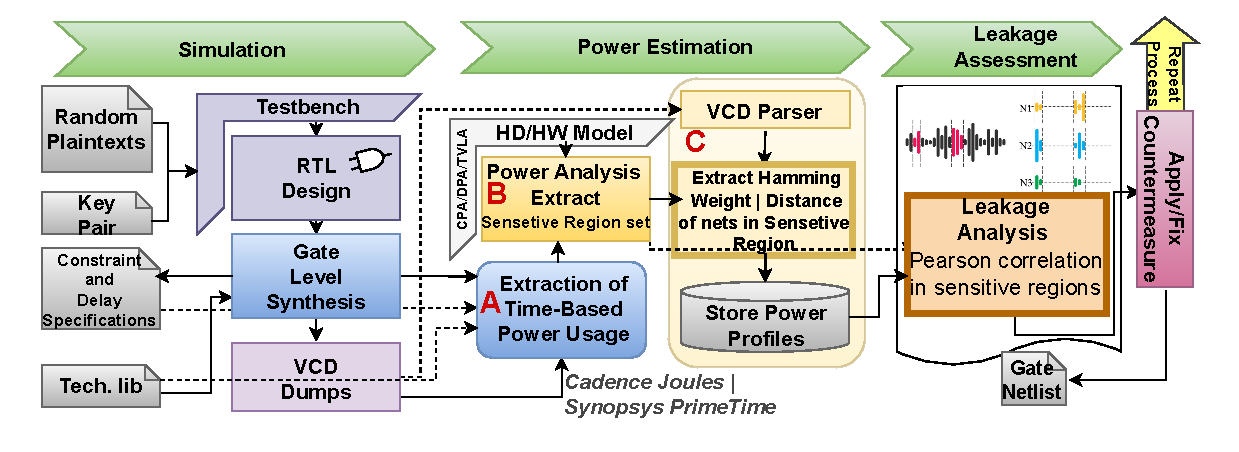
\includegraphics[width=0.5\textwidth]{Pictures/PATHbold.pdf}
     \caption{The PATCH methodology, based on the description in
     ~\cite{PATCH}.}
     \label{fig:patch}
 \end{figure}
PATCH is a gate-level methodology for pinpointing PSC vulnerabilities, using the netlist of a design, by correlating each net’s toggling activity with a HD/HW power model. 
Operating at the gate-level abstraction, PATCH relies on toggling statistics that inherently incorporate real gate delays and glitches. Fig.~\ref{fig:patch} illustrates PATCH w.r.t. the three aforementioned phases.



\noindent{\bf Simulation. }
A gate-level netlist is obtained from the synthesized design, together with technology-specific constraints (SDC/SDF files). 
The design is then simulated with multiple plaintext inputs to produce VCD files, accurately accounting for timing delays.

\noindent{\bf Power Estimation. }
First, a CPT leverages the netlist, timing data, and technology libraries to generate time-series power traces for every VCD file (step \emph{A} in Fig.~\ref{fig:patch}). Next, leakage analysis techniques such as Differential Power Analysis (DPA), Correlation Power Analysis (CPA), or T-tests \cite{bluebook} detect time windows, called \emph{sensitive regions}, during which the design is most vulnerable (step \emph{B}). Finally, a dedicated VCD parser tracks toggles on every net in the sensitive regions, estimates net-level dynamic power consumption using a HD/HW model, and stores the power profiles (step \emph{C}).

\noindent{\bf Leakage Assessment. }
Within the sensitive regions, the net-level power traces are individually correlated against the total design power consumption to identify nets that most significantly contribute to leakage. A high correlation implies that modifying these nets' switching behavior or applying localized countermeasures may substantially reduce side-channel attack vulnerability. Designers can then selectively harden the nets with high correlation to meet their acceptable leakage level.


\subsection{ACA: Architecture Correlation Analysis}\label{sec:ACA}

 \begin{figure}[!t]
     \centering
     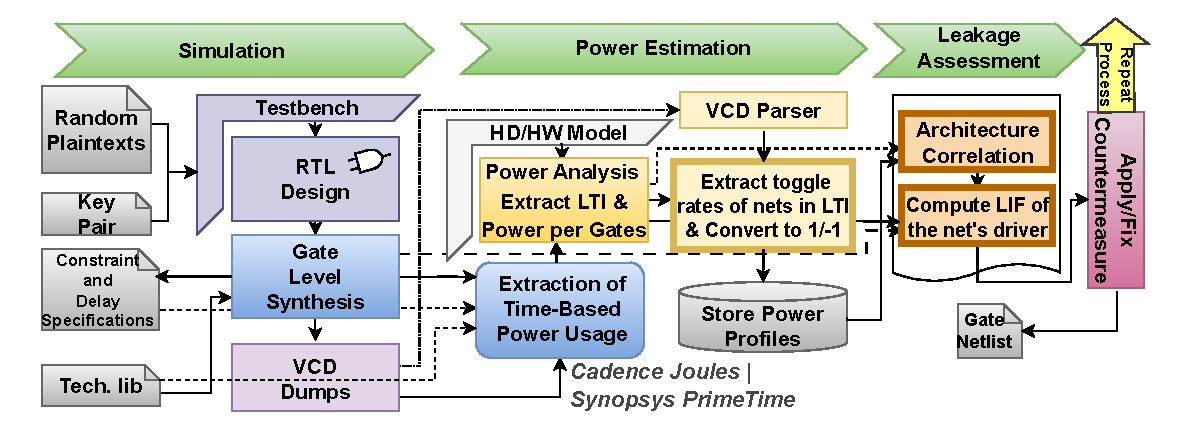
\includegraphics[width=0.5\textwidth]{Pictures/ACA2.pdf}
     \caption{ACA methodology, based on the description in~\cite{ACA}.}
     \label{fig:ACA}
     \vspace{-2mm}
 \end{figure}


ACA is a design-time methodology intended to identify which gates in a gate-level netlist contribute the most to side-channel leakage. Three inputs are required: (1) a gate-level netlist, (2) a known leakage model \(L(V)\) 
where the leakage model \(L\)
is a function computed over a secret intermediate variable \(V\), and (3) time-series power traces obtained from stimuli that exercise the secret variable \(V\). Once these are available, ACA proceeds with the three main phases shown in Fig.~\ref{fig:ACA}.

\noindent{\bf Simulation. } Similar to PATCH, a gate-level simulation is performed on the netlist (along with SDF/SDC files). Various plaintexts or input stimuli are applied, and each net's toggling activity is recorded in VCD files.

\noindent{\bf Power Estimation. }
After generating power traces using a CPT, ACA determines a \emph{Leakage Time Interval (LTI)} by correlating the total power consumption \(P(t)\) with the leakage model \(L(V)\) as:
\begin{equation}
\rho_{L(V),t}=\frac{\operatorname{cov}\!\big(L(V),P(t)\big)}{\sigma_{L(V)}\,\sigma_{P}},
  \label{eq:ACA_1}
\end{equation}
\noindent%\small
where \(\operatorname{cov}\) is the covariance operation, and \(\sigma_{L(V)}\) and \(\sigma_{P}\) are the standard deviations of \(L(V)\) and \(P\), respectively.
Any time window in which \(\rho_{L(V),t}\) exceeds the Pearson correlation threshold (as defined under the "Pearson correlation Threshold" section of Table~\ref{tab:confidence}, depending on the chosen confidence level and sample size) is treated as containing meaningful leakage and constitutes the LTI. While determining the LTI, the CPT also provides gate-level average power data for subsequent analysis.

\noindent{\bf Leakage Assessment. } \label{sec:ACA_leak}
Within each LTI, ACA computes an \emph{architecture correlation factor} \(C_i\) for every net \(i\). Let \(K_i\) be the \emph{toggle trace} of net \(i\), with \(+1\) if the net toggles and \(-1\) otherwise, and the toggle trace of the leakage model is \(H\). The correlation factor is computed as the dot product (Eq.~\ref{eq:ACA_3}) -- see Table~\ref{tab:example_AC} for a simple example using stimuli \(S_0\)–\(S_3\). Subsequently, the \emph{LIF} \(F_i\) is defined by scaling \(C_i\) with the gate’s average power consumption in the LTI (Eq. ~\ref{eq:ACA_4}).

\noindent
\begin{minipage}{0.48\linewidth}
\begin{equation}
  C_i = K_i \cdot H
  \label{eq:ACA_3}
\end{equation}
\end{minipage}\hfill
\begin{minipage}{0.48\linewidth}
\begin{equation}
  F_i = C_i\,\frac{P_i}{P_T}
  \label{eq:ACA_4}
\end{equation}
\end{minipage}
\noindent
Here, \(P_i\) is the average power consumption of the gate driving net \(i\) within the LTI, and \(P_T\) is the design’s total power over that interval. Larger \(F_i\) flags gates whose toggling aligns with the model and that draw significant power. ACA ranks gates by \(F_i\) to prioritize and apply countermeasures.

{
\renewcommand{\arraystretch}{0.9}

\begin{table*}[t]
\centering
\footnotesize
\setlength{\tabcolsep}{8pt}
\caption{Thresholds for statistical estimators used by RTL-PAT~\cite{RTL_PSC} and ACA~\cite{ACA}.}
\label{tab:confidence}

\begin{tabular*}{\textwidth}{@{\extracolsep{\fill}}cc|cc|c|ccc@{}}
\toprule
\multicolumn{4}{c|}{\textbf{KL Divergence Threshold}} &
\multicolumn{4}{c}{\textbf{Pearson Correlation Threshold}} \\
\cmidrule(lr){1-4}\cmidrule(lr){5-8}
\textbf{$P_r$} & \textbf{KL} &
\textbf{$P_r$} & \textbf{KL} &
\textbf{Confidence Interval} &
\textbf{n=600} & \textbf{n=1000} & \textbf{n=2000} \\
\midrule
$>0.96$ & $<0.01$ & $>0.61$ & $<0.50$ &
99\% & $\pm0.105$ & $\pm0.081$ & $\pm0.058$ \\
$>0.90$ & $<0.03$ & $>0.45$ & $<1.12$ &
95\% & $\pm0.080$ & $\pm0.062$ & $\pm0.044$ \\
$>0.80$ & $<0.12$ & $>0.32$ & $<2.00$ &
90\% & $\pm0.067$ & $\pm0.052$ & $\pm0.037$ \\
\bottomrule
\end{tabular*}
\end{table*}

}


\section{Common Evaluation Framework and Comparison.}
\label{sec:comparison}
To compare the three pre‑silicon methodologies, introduced in Section~\ref{sec:Comparative},  under identical conditions, we built a
moderately complex benchmark around the open‑source
Ibex 32‑bit RISC‑V core
\cite{8106976}.  Ibex is written in SystemVerilog and supports the RV32I/E, M, C
and B extensions.  A software implementation of AES‑128
(\emph{Tiny‑AES}~\cite{kokke_tinyAESc2024}) executes on the core and
generates the switching activity within the core hardware structure that is analyzed by each methodology.  The Ibex design was
synthesized using the \mbox{GF\textsuperscript{\textregistered}
22FDX} technology (Genus 21.14) and contains \(\approx\!8\text{K}\) gates which are driving nets, with 10 MHz clock frequency.
In the following, we compare how long each methodology takes to analyze the Ibex design, i.e., its computational runtime overhead.

We implemented the three methodologies in Python\footnote{The source code and scripts  available at: \url{https://github.com/abolfazlsajadi/ASSESS}} and their analysis phases were executed on
the same workstation (Intel Core i7, 8 cores, 32 GB RAM) to ensure fair comparison  of the methodologies' runtime
and memory requirements.  
Since the power trace generation is both multi threaded and memory intensive, it was carried out on a separate server equipped with an AMD Ryzen 9 3900X
(12 cores, 128 GB RAM) and a large local storage. The power traces were sampled every 25 ns, i.e., four samples per 100 ns clock period, matching the timing resolution required by all methodologies. Power estimates were obtained with CPT (Cadence\textsuperscript{\tiny®} Joules) using the GF 22FDX standard-cell library, while side-channel analyses were carried out with the ChipWhisperer Analyzer \cite{o2014chipwhisperer}.
Using these CPT generated traces, a correlation power analysis (CPA) under the Hamming-Weight leakage model revealed all 16 Tiny-AES key bytes with only 45 traces \cite{o2014chipwhisperer,bluebook}.
\label{sec:rtlpsc_ibex}

 
\subsection{The RTL‑PAT Methodology on Ibex}

The RTL‑PAT methodology, described in Section~\ref{sec:RTL‑PAT}, requires two cryptographic keys to compare their switching activity distributions. A naive all‑zero vs.\ all‑one pair, as suggested in the original paper \cite{RTL_PSC}, cannot be used on Ibex, since the multiply/divide unit detects a division by zero in the first cycle and terminates execution. To preserve a high Hamming distance and constant‑time execution, we instead use the two fixed key patterns \texttt{00\,FF\,00\,FF…} and \texttt{FF\,00\,FF\,00…} . For each key, we record 500 VCD files (by QuestaSim). Each trace covers 10K clock cycles sampled twice per cycle, yielding 20K time samples per trace for the leakage evaluation.

\begin{table}[!b]
\centering
\caption{RTL-PAT end-to-end runtime ($500\times2$ traces).}
\label{tab:pscrtl_timing}

%\begin{tabularx}{\columnwidth}{l l X c}
\begin{tabular}{l| l p{0.34\columnwidth} c}
\hline
\textbf{Phases} & \textbf{Step} & 
\textbf{Per trace / once} & \textbf{Total} \\ \hline

%\multicolumn{1}{l|}{\multirow{2}{*}{Sim.}} 
%& Vmem gen. & 141ms & 2m\,24s \\
%\multicolumn{1}{l|}{} 
%& VCD dump & 4.43s & 1h\,16m \\ \hline
\multirow{2}{*}{Sim.} & Vmem gen. & 141ms & 2m\,24s \\
& VCD dump & 4.43s & 1h\,16m \\ \hline

\multirow{2}{*}{Pwr.\ Est.} 
& VCD parsing$^{\mathrm{1}}$ & 16.6s & 4h\,36m \\
{} 
& VCD parsing$^{\mathrm{2}}$ & 2.39s & 41m\,39s \\ \hline

Lkg.A. 
& $D_{KL}$ divergence & 3.13s & 3.13s \\ \hline

\multicolumn{2}{l}{end-to-end runtime$^{\mathrm{1}}$} & & 5h\,54m \\
\multicolumn{2}{l}{end-to-end runtime$^{\mathrm{2}}$} & & 2h\,6s \\ \hline

\multicolumn{4}{l}{1: single-thread \quad 2: multi-thread (16)}
\end{tabular}%\end{tabularx}
\end{table}



Fig.~\ref{fig:rtlpsc_ibex} depicts the 37 Ibex modules, grouped into plots by their $D_{KL}$ divergence, and reports their cycle-by-cycle leakage.  Because RTL-PAT analyzes only entire modules, it cannot pinpoint which nets inside a module are responsible for the leakage, and a large $D_{KL}$ value does not automatically imply an exploitable vulnerability.
Table~\ref{tab:pscrtl_timing} shows a breakdown of the RTL-PAT runtime. The overwhelming bottleneck is the VCD parsing. However, parallelizing the gathering transitions stage (VCD parsing) reduces the end-to-end run time from almost six hours to about two hours. The $D_{KL}$ divergence computation itself requires only a few seconds. Although Ibex is smaller than a full multi-core SoC, it is a realistic synthesized RISC-V core that serves as a common benchmark for all three methodologies and for our RTL-PAT optimization. However, because RTL-PAT detects leakage only at the coarse granularity of modules, we next turn to gate-level techniques that can localize vulnerable logic more precisely.

\subsection{The PATCH Methodology on Ibex}
\label{sec:PATCH_ibex}

Unlike RTL-based approaches, PATCH leverages gate-level information. 
Fig.~\ref{fig:patch2} shows the CPA results, with the highest correlation for each key byte highlighted. 
The x-axis denotes the sample index; traces are sampled every 25\,ns (four samples per 10\,MHz clock cycle). 
We first identify \emph{sensitive regions}, i.e., indices with significant leakage, and expand each by ±20 neighbouring samples ($\approx$±5 clock cycles) to form \emph{sensitive regions}. 
Within these regions, we analyze the net switching activity and compute the Pearson correlation against the HW model.
 \begin{figure}[b]
     \centering
     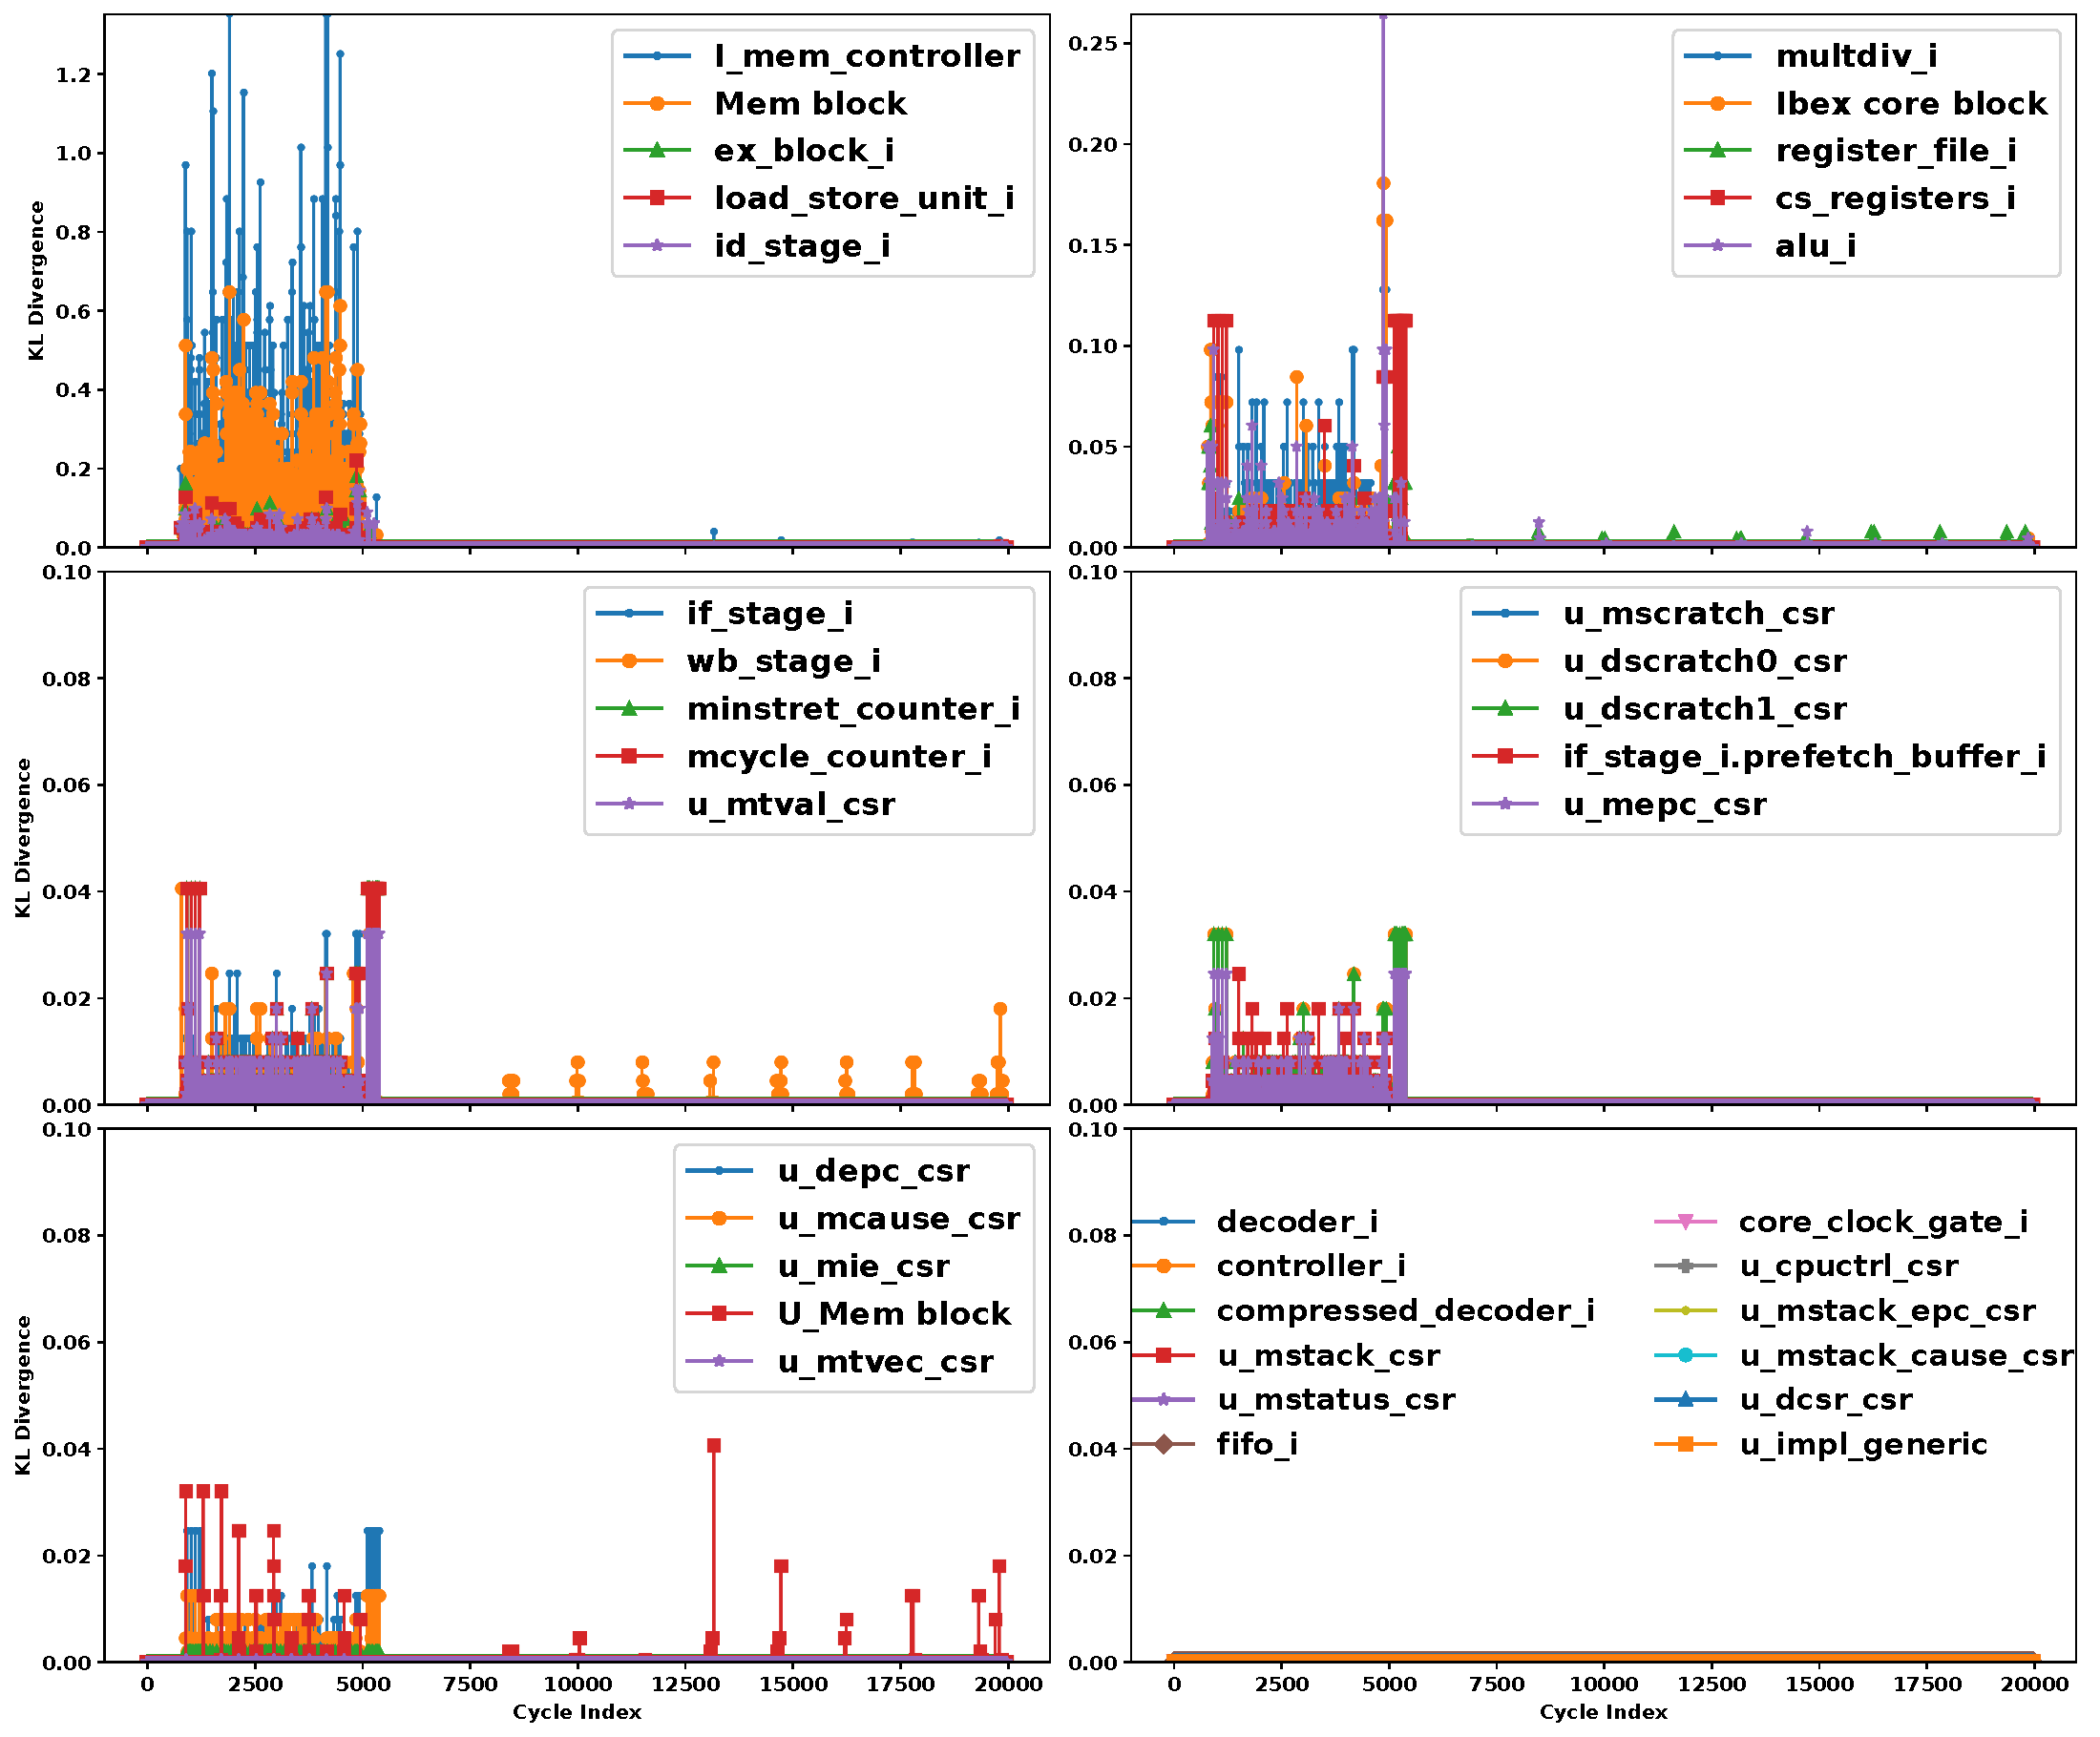
\includegraphics[width=\columnwidth]{Pictures/kl_2x3_fplot_optimized.pdf} %vector is PDF
     \caption{Results of the RTL-PAT method on Tiny-AES running on an Ibex core.}
     \Description{Plot of KL divergence over traces for Tiny-AES running on Ibex using RTL-PAT methodology.}
     \label{fig:rtlpsc_ibex}
 \end{figure}
\begin{figure}[!t]
    \centering
    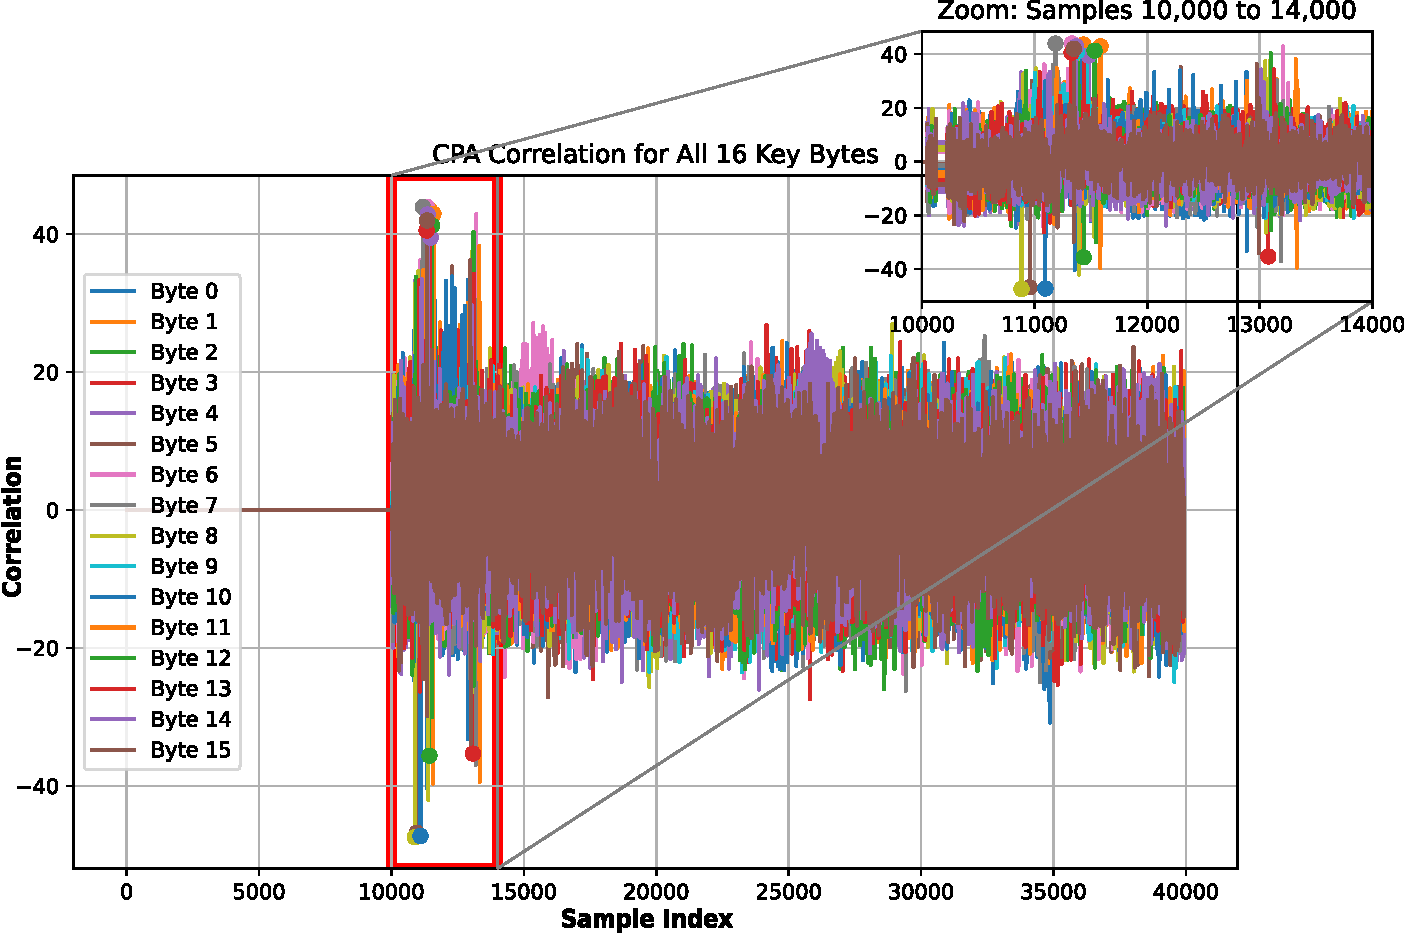
\includegraphics[width=\columnwidth]{Pictures/PATH_2x3_plot24.pdf}
    \caption{CPA per key byte (600 traces) with peaks marking sensitive moments.}
    \label{fig:patch2}
    \vspace{-2mm}
\end{figure}

Fig.~\ref{fig:patchresults_ibex} shows the distribution of absolute Pearson correlations between each net and the HW model for all 16 key bytes. The x-axis groups $|r|$ into four ranges, and the y-axis (log scale) reports how many nets fall into each range. Each bar corresponds to one key byte index. For all key bytes, the vast majority of nets have low correlation ($|r| < 0.5$), while only a small fraction reach the highest bin ($0.8 \le |r| \le 1.0$). Across the $\sim 8$k nets in Ibex, fewer than $10^{3}$ nets exceed $|r| > 0.8$, so PATCH reduces the set of nets that require detailed inspection from the full design to this much smaller subset of highly correlated candidates.


\begin{figure}[t]
    \centering
%    \vspace{-5mm}
    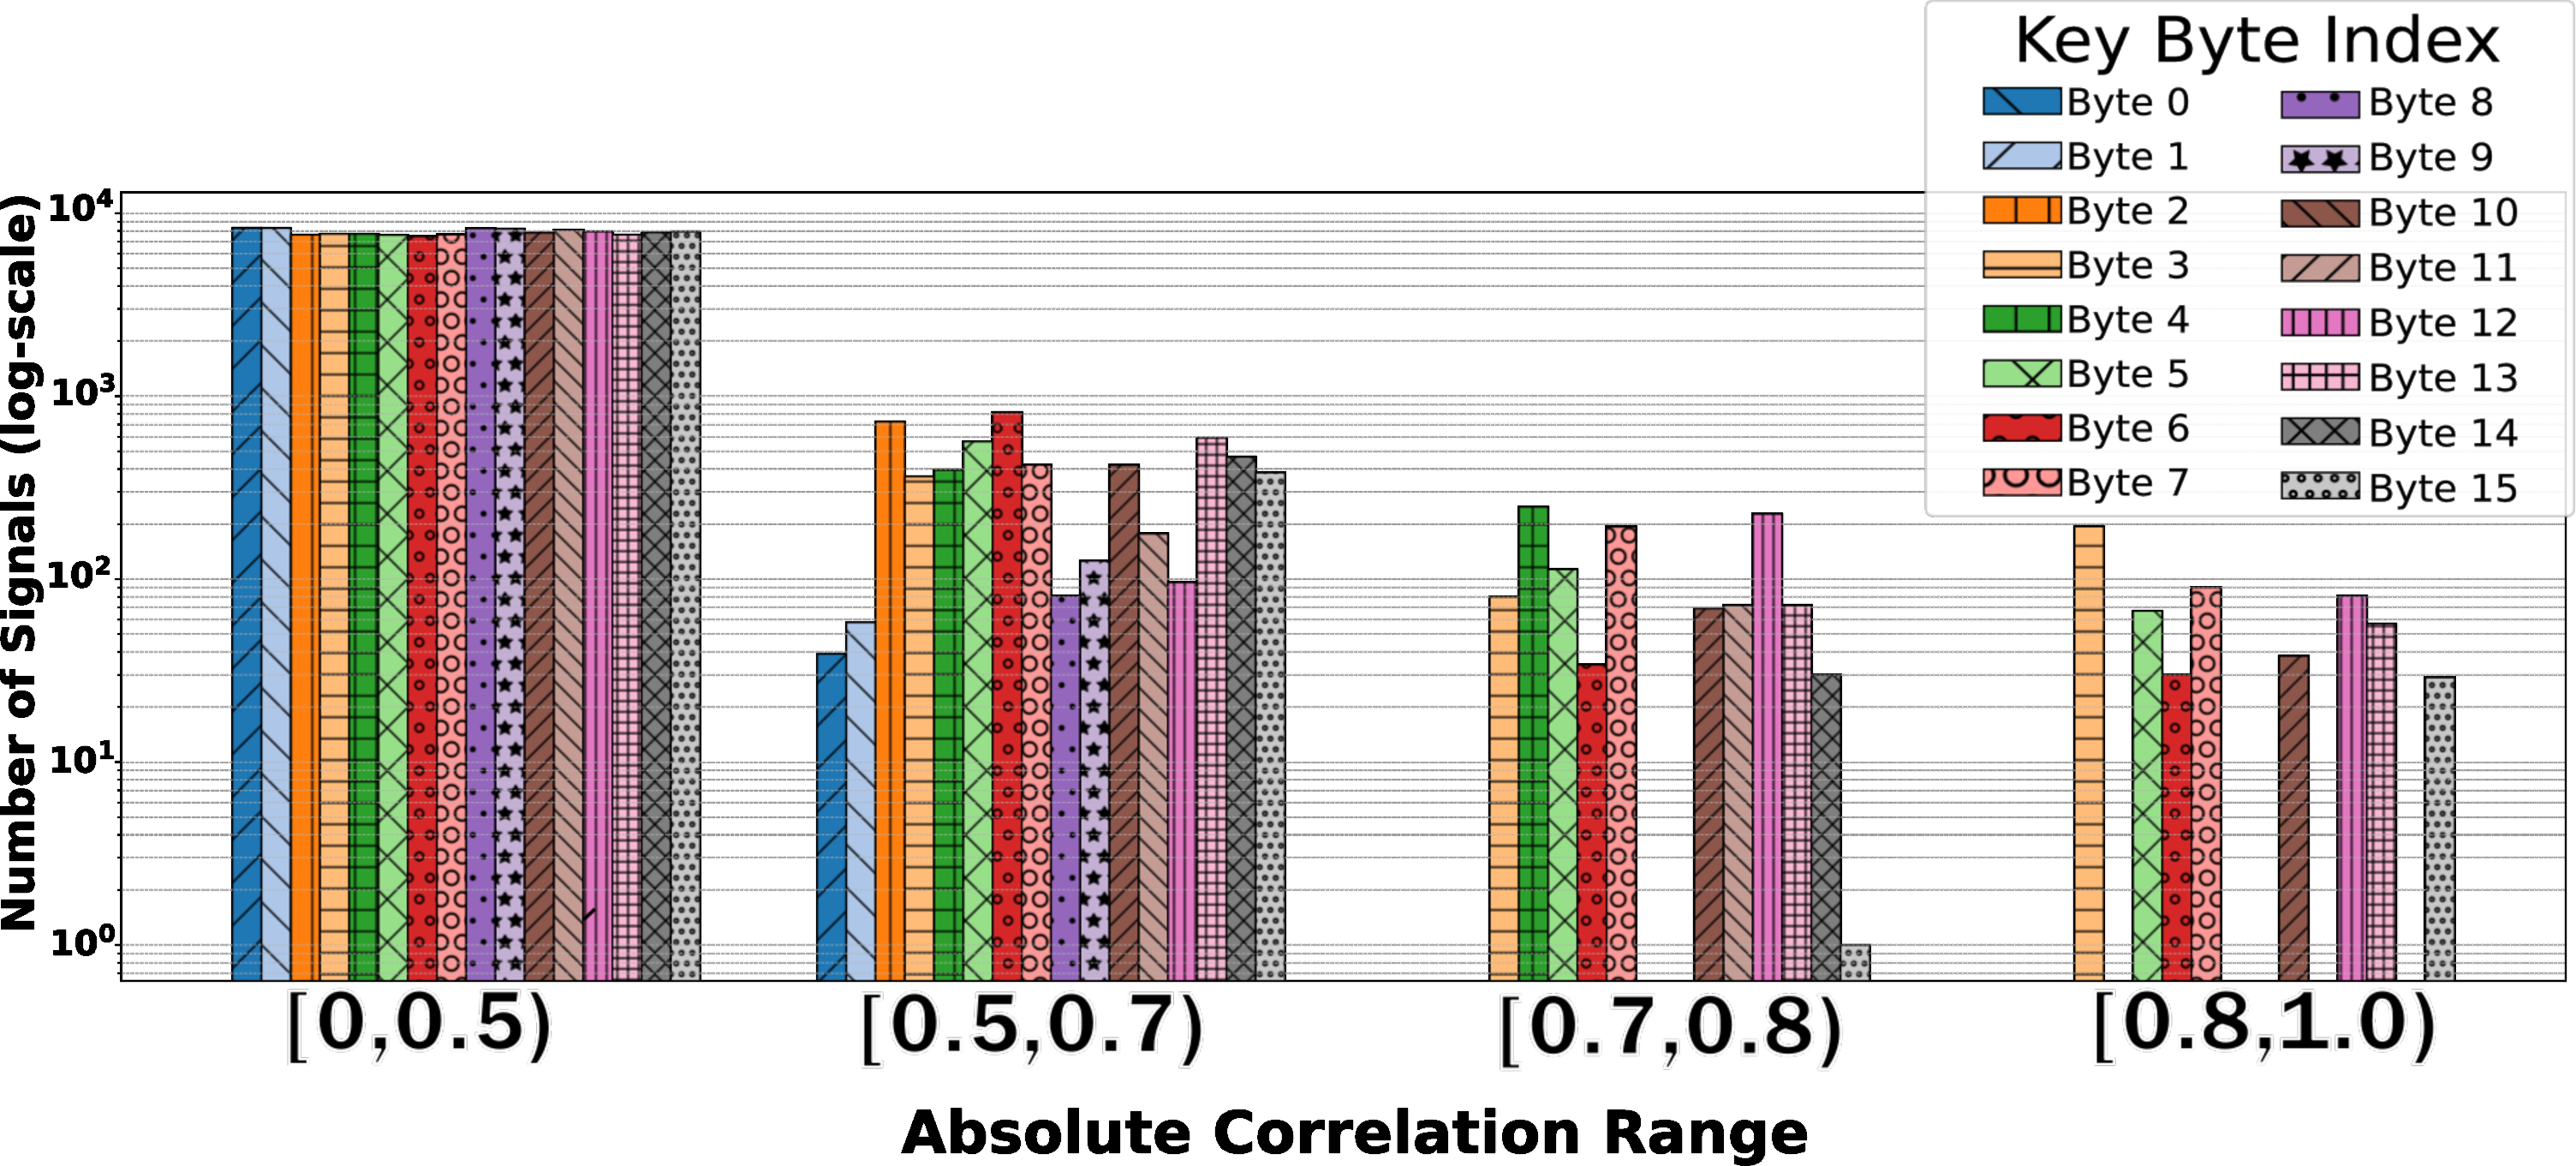
\includegraphics[width=1\columnwidth]{Pictures/b1yte_correlation_distributiongggg.pdf}
    \caption{Distribution of signal correlations with the HW-based key bytes.}
    \label{fig:patchresults_ibex}
    \vspace{-1mm}
\end{figure}
Table~\ref{tab:patchruntime_breakdown} shows a breakdown of the PATCH runtime. The dominant cost is the power extraction with CPT (about 72 days), followed by gate-level simulation \(\approx1\ hour\) and the original net-activity parsing \(\approx13\ hours\). According to the PATCH reference flow (Fig.~\ref{fig:patch}), the net activity is usually extracted from the entire VCD file before isolating sensitive regions, which becomes memory-intensive for large designs and prevents multi-threading.  
To optimize this, we extract the net activity only within the sensitive regions, reducing the required memory by \(\approx97\%\). Without region reduction, processing the full design requires 78.7 s/trace. When restricted to the reduced sensitive regions, the runtime decreases to 16.4 s/trace using a single thread and further to 0.86 s/trace with 16 threads, resulting in an overall time saving of \(\approx13\ hours\) hours across 600 traces.\looseness=-1
\begin{table}[]
\centering
\caption{PATCH end-to-end runtime (600 traces).}
\label{tab:patchruntime_breakdown}

%\begin{tabularx}{\columnwidth}{l l X c}
\begin{tabular}{l| l p{0.25\columnwidth} c}
\hline
\textbf{Phases} & \textbf{Step} &
\textbf{Per trace} & \textbf{Total} \\ \hline

\multirow{3}{*}{Sim.}
& Vmem gen. & 141ms & 1m\,24s \\
{}
& Synthesis (once) & -- & 5m\,53s \\
{}
& VCD dump & 6.32s & 1h\,03m \\ \hline

\multirow{2}{*}{Pwr.\ Est.}
& Power extraction & 2h\,54m\,26s & 72d\,15h\,36m \\
{}
& VCD parsing & 78.7s & 13h\,7m \\ \hline

Lkg.A.
& Pearson’s $\rho$ (16B) & 23.4s & 3h\,53m\,36s \\ \hline

\multicolumn{2}{l}{end-to-end runtime} & & \textbf{73d\,6h\,22m} \\ \hline
\end{tabular}%\end{tabularx}
\vspace{-1mm}
\end{table}



The authors of PATCH evaluated a fully unrolled AES implementation (coprocessor) \cite{unrolledAED} but did not disclose the technology node.  Our experiments with a 22nm library did not result in a similar timing as theirs, even though the design was comparable. The difference most likely stems from different technology libraries, delay models, sampling resolutions, or EDA tools (for CPT they used PrimeTime PX; we used Joules). In our own experiments, we quantified this effect by synthesizing the same fully unrolled AES coprocessor~\cite{unrolledAED} using two standard-cell libraries that differ only in technology node, thereby illustrating the impact of the chosen/target technology on the runtime of this methodology.
\begin{itemize}[leftmargin=1.5em, nosep]
  \item With a $0.18\,\mu\text{m}$ library, synthesis finished in 120 s and CPT needed 1 min 04 s to generate a single power trace.

   \item Retargeting the identical RTL and tool settings to a 22nm library stretched synthesis time to 811 s, while power trace generation ballooned to 54 min 44 s per trace.
\end{itemize}
The order-of-magnitude slow-down can mainly be explained by the richer timing and power-characterization formats used at advanced nodes which drive both larger libraries and finer-grained delay/power interpolation within CPT. Consequently, it is important to report the technology node alongside the design complexity and sampling rate when comparing power analysis runtimes for hardware side-channel studies.

Because the leakage model compares the activity of individual nets against byte-level differences and does not account for the net’s physical location or the identity of its driving gate, some false positives remain. That is, certain nets, such as primary inputs, may appear correlated with the leakage model despite having minimal impact on the overall power consumption. Nevertheless, this approach significantly narrows down the candidate set compared to blanket countermeasures. This motivates a finer-grained analysis in the form of a per-gate ranking method known as ACA, which we examine next.

%%%%%%%%%%%%%%%%%%%%%%%%%%%%%%%%%%%%%%%%%%%%%%%%%%%%

%--------------------------------------------------------------------%
\subsection{The ACA Methodology on Ibex and {AES coprocessor}}
\label{sec:ACA_ibex}
%--------------------------------------------------------------------%
In this section, we evaluate the performance of ACA not only on Ibex running Tiny-AES but also on a stand-alone hardware module, namely an AES coprocessor. This extra evaluation enables more thorough comparison of ACA with our \methodname\ methodology presented in Section~\ref{sec:Methodology}. The AES coprocessor implements AES-128 with on-line key expansion and completes one encryption in 11 clock cycles. The coprocessor design does not include dedicated side-channel countermeasures and is available as an RTL Verilog implementation~\cite{projectvault_aes_verilog}.
\begin{figure*}[!t]
  \centering
  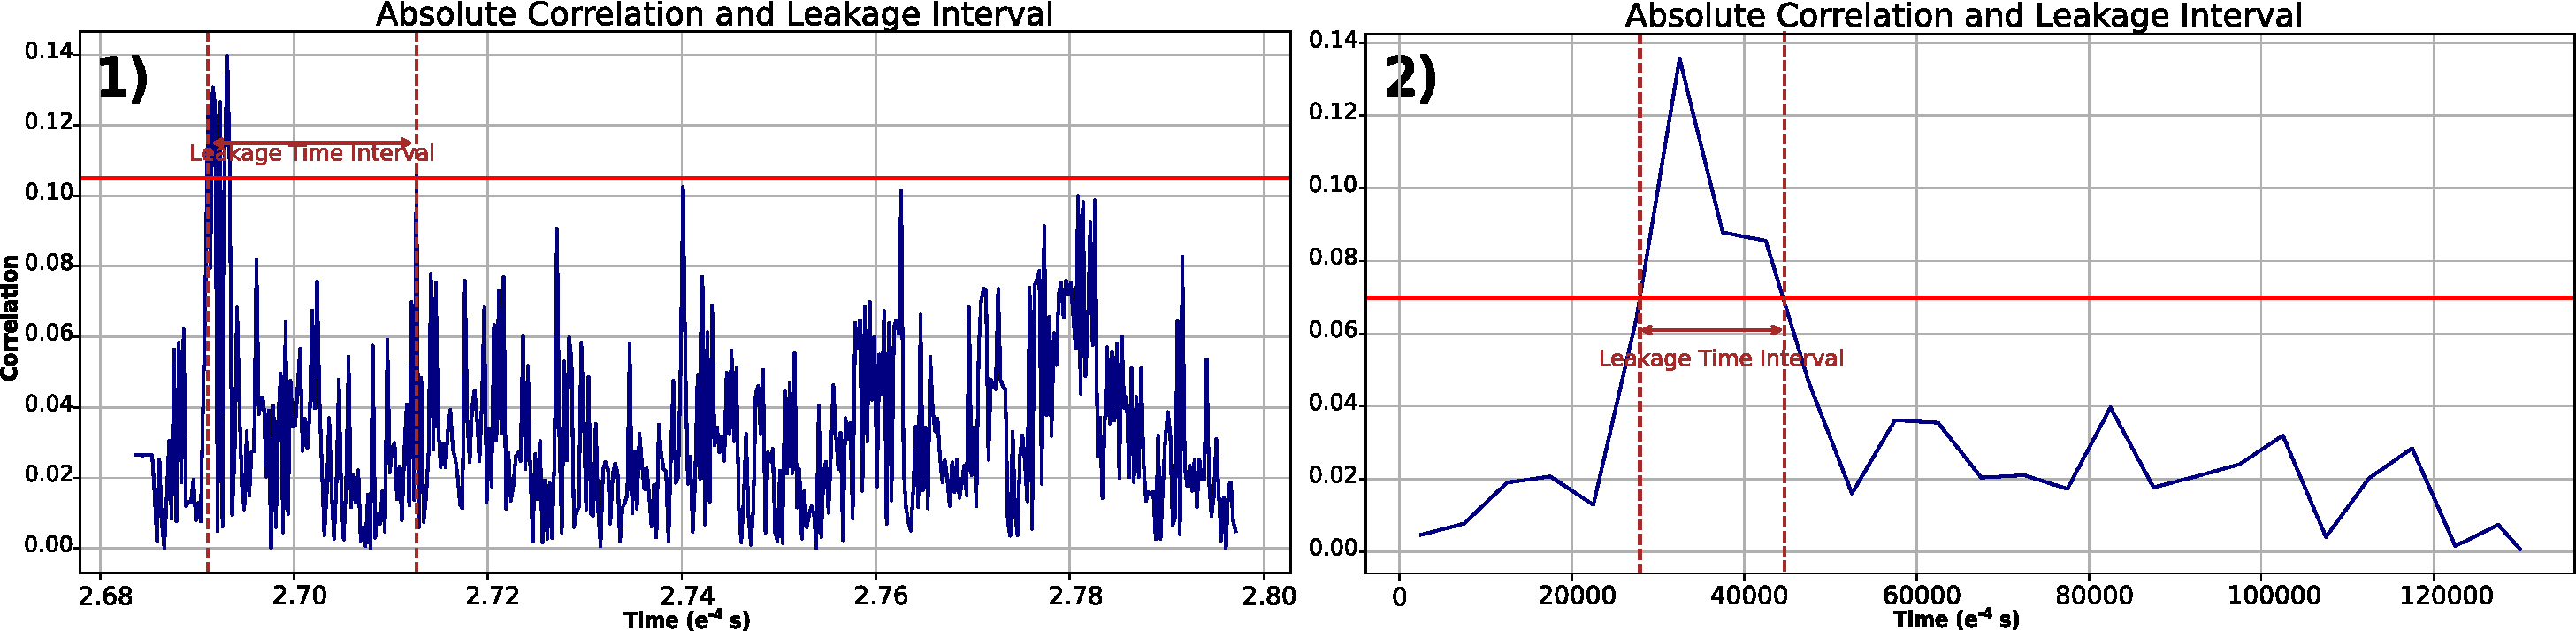
\includegraphics[width=1.9\columnwidth]{Pictures/ACA_correlation_distributionnew13.pdf}
  \caption{LTI obtained for first S-box Tiny-AES state bit 0 correlation 1) using 600 traces on Ibex (zoomed-in); 2) using 1500 traces on AES coprocessor. }%($|\rho|=0.105$);
  \label{fig:ACA_corr50}
\end{figure*}

% Leakage interval from first 99\% peak 
\noindent{\bf Methodology and leakage model.}
Following the original ACA study~\cite{ACA} (summarized in Section~\ref{sec:ACA}), we adopt the HD leakage model, where each elements corresponds to the HD between two consecutive values of the 128-bit Tiny-AES state register. Fig.~\ref{fig:ACA_corr50}(1) shows a zoom-in on the first S-box execution and the corresponding Pearson correlation (Eq.\,(\ref{eq:ACA_1})), computed from an initial set of 600 input patterns. The dominant peak clearly identifies the prospective LTI, with a correlation magnitude of \(\rho_{L(V),t}\approx 0.14\), which exceeds the 99\,\% confidence threshold of \(0.105\) (red line) for 600 traces (Table~\ref{tab:confidence}). This confirms both the suitability of the HD model and the correctness of the chosen LTI.  Fig.~\ref{fig:ACA_corr50}(2) shows the Pearson correlation for the 11-cycle AES coprocessor (including two additional cycles for data loading and result readout). With 1500 traces, we obtained \(\rho_{L(V),t}\approx 0.13\), which is above the 99\,\% confidence threshold of \(0.069\) (red line).
\begin{table}[t]
\centering
\caption{Example of Architecture Correlation}
\label{tab:example_AC}
\begin{tabular}{@{}lccccr@{}}
\toprule
 & S0 & S1 & S2 & S3 & $C_{ij}$ \\
\midrule
\textbf{Leakage Model (H$_j$)} & $+1$ & $-1$ & $-1$ & $+1$ & \\
\textbf{net0 (K$_0$)} & $+1$ & $-1$ & $-1$ & $+1$ & $4$ \\
\textbf{net1 (K$_1$)} & $+1$ & $+1$ & $+1$ & $+1$ & $0$ \\
\textbf{net2 (K$_2$)} & $-1$ & $-1$ & $+1$ & $-1$ & $-2$ \\
\bottomrule
\end{tabular}
\end{table}
\noindent{\bf Deriving the LIF distribution.} After recording the toggle trace for every net \(i\) within each LTI
(Section~\ref{sec:ACA}), we compute the \emph{architecture correlation}
\(C_i\) with the dot product of Eq.\,(\ref{eq:ACA_3}); this measures the
functional dependency between net \(i\) and the leakage model H.
A large Pearson coefficient in Eq.\,(\ref{eq:ACA_1}) indicates that the
\emph{total} power follows the model, whereas a large \(C_i\) pinpoints
the \emph{individual} net that responsible for it.
Following~\cite{ACA}, we traverse the netlist to locate the gate that
drives each net \(i\). Each drivers average power \(P_i\) is obtained from 
the CPT and then normalized by the design-wide mean power
\(P_T\) to obtain the \emph{leakage-impact factor} \(F_i\) in Eq.\,(\ref{eq:ACA_4}). 
The gates with the highest \(F_i\) contribute the most to side-channel leakage, 
which enables ACA to rank their relative impact on the overall power-leakage footprint.

\begin{figure}[!t]
  \centering
  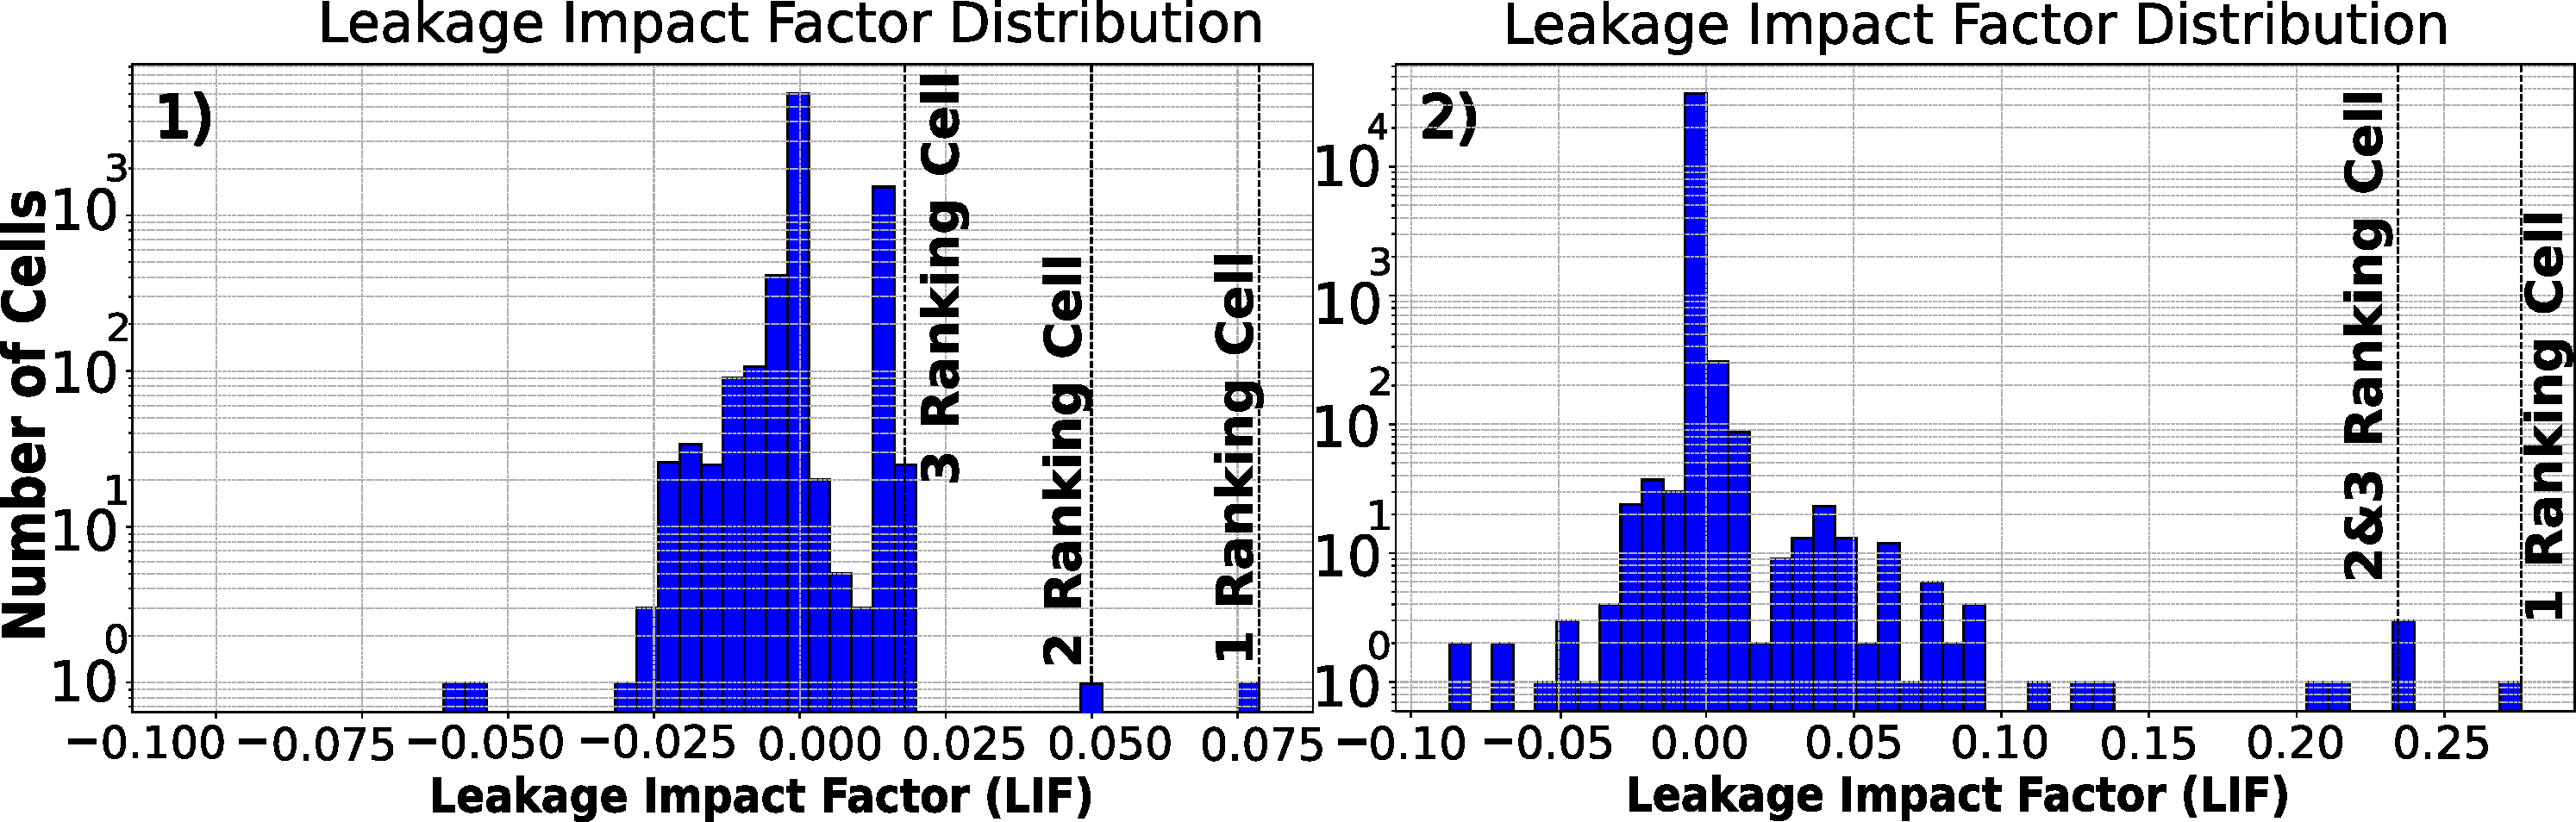
\includegraphics[width=\columnwidth]{Pictures/dualNETLIF_distributionnew.pdf}
  \caption{
  ACA LIF distribution for  
  1) 600 traces on Ibex; and 2) 1500 traces on AES coprocessor (log scale).}
  \label{fig:ACA_LIF600}
  \vspace{-2mm}
\end{figure}

Fig.~\ref{fig:ACA_LIF600} illustrates the LIF distribution for all gates in both the Ibex design executing Tiny-AES (part~1) and the AES coprocessor (part~2), as obtained from the ACA output. In both cases, the distribution is strongly skewed: only a small fraction of gates exhibit large LIF values, meaning that a few gates dominate the side-channel leakage predicted by the chosen model. The results show that the top-ranked element in both cases is the AES state bit 0: a flip-flop in the Ibex register file and a flip-flop in the coprocessors internal state for AES block.   
In both designs, these registers toggle after every AES round, making them the most active and consequently the leakiest components. The next highest entries correspond to gates within the S-box logic directly driven by the state register outputs. Beyond these, the LIF values drop sharply, indicating that the remaining gates contribute only marginally to the overall side-channel leakage.\\
%%%%%%%%%% 
\noindent{\bf Runtime of the reference ACA flow. } Table~\ref{tab:runtime_breakdown_ACA} reports the end-to-end runtime for the ACA methodology of~\cite{ACA}. The dominant bottleneck of ACA is the power extraction step performed with CPT, which generates full gate-level power traces. For the Ibex core, this step requires approximately 2.9\,hours per trace, resulting in a total runtime of about 72\,days for 600 traces. All other phases of the methodology (correlation, VCD parsing, and netlist analysis) together add only about three additional hours. In contrast, for the AES coprocessor, the total power extraction time is significantly shorter: roughly 18\,seconds per trace (7.5\,hours total for 1500 traces), owing to the lower number of clock cycles (two samples per clock).    

{
\renewcommand{\arraystretch}{0.9}

\begin{table*}[t]
\centering
\setlength{\tabcolsep}{8pt}
\caption{ACA runtime breakdown for the Ibex and AES coprocessor.}
\label{tab:runtime_breakdown_ACA}

\begin{tabular}{l|p{0.37\textwidth}cccc}%\begin{tabularx}{\textwidth}{l|Xcccc}
\hline
\multicolumn{2}{c}{} &
\multicolumn{2}{c}{\textbf{Ibex (600 traces)}} &
\multicolumn{2}{c}{\textbf{AES coprocessor (1500 traces)}} \\
\cline{3-6}
\textbf{Phases} & \textbf{Step} &
\textbf{Per-trace} & \textbf{Total} &
\textbf{Per-trace} & \textbf{Total} \\ \hline

\multirow{3}{*}{Sim.}
& Vmem generation        & 141\,ms      & 1\,m\,24\,s   & —            & — \\
{}
& Synthesis (once)       & —            & 5\,m\,53\,s   & —            & 36\,m\,9\,s \\
{}
& VCD dump               & 6.32\,s      & 1\,h\,3\,m    & 3\,s         & 1\,h\,15\,m \\ \hline
\rowcolor{LightGray}
\multirow{4}{*}{Pwr.\ Est.}
& Power extraction
%%\multicolumn{1}{l|}{\multirow{4}{*}{Pwr.\ Est.}}
%%& \rowcolor{LightGray} Power extraction
                         & 2\,h\,55\,m  & 72\,d\,15\,h  & 18\,s        & 7\,h\,30\,m \\
{}
& Power analysis (HD)    & —            & 13\,s         & —            & 10\,s \\
{}
& VCD parsing            & 2.5\,s       & 25\,m         & 3.47\,it/s   & 7\,m\,12\,s \\
{}
& Per-gate power scan (Joules)
                         & —            & 19\,s         & —            & 2\,m\,49\,s \\ \hline

Lkg.A.
& Net-list parsing \& LIF & 40\,nets/s   & 3\,m\,28\,s   & 12.5\,nets/s & 50\,m\,12\,s \\ \hline

\multicolumn{2}{l}{end-to-end runtime}
&  & \textbf{72\,d\,15\,h\,31\,m}
&  & \textbf{10\,h\,22\,m} \\ \hline
\end{tabular}%\end{tabularx}
\end{table*}

}


\noindent{\bf Sampling-rate versus runtime.} 
In our experiments, we used CPT (Cadence Joules) with a sampling rate of four samples per clock cycle (25\,ns/sample on a 100\,ns period) for the Ibex core and two samples per clock cycle (5\,ns/sample on a 10\,ns period) for the AES coprocessor, ensuring that glitches and intra-cycle delays are fully captured. Even when using a lower sampling rate, the power extraction step remains the dominant contributor to the total runtime. The timing results for Ibex are as follows:
\begin{itemize}[leftmargin=1.5em, nosep]%\itemsep=0pt \parsep=0pt \topsep=0pt
  \item 2~samples/cycle: 1\,h\,14\,min per trace  
        \(\rightarrow\) 31\,days for 600 traces;
  \item 1~sample/cycle: 29\,min per trace  
        \(\rightarrow\) 12\,days for 600 traces;
  \item 1~sample/2~cycles: 16\,min per trace  
        \(\rightarrow\) 7\,days for 600 traces.
\end{itemize}
Thus, although accuracy can be traded for speed, power extraction remains the dominant bottleneck in ACA—particularly when frequent back-end revisions (e.g., new technology corners) necessitate a full re-run.\\



\noindent{\bf Comparison and key observations. }The last three columns in Table~\ref{tab:comparison} summarize the main features of the RTL-PAT, PATCH, and ACA methodologies. RTL-PAT operates at a higher level of abstraction (RTL), compared to PATCH and ACA. This leads to much shorter end-to-end runtime, e.g., $\approx 2$ hours for the Ibex benchmark, and eliminates dependencies on technology libraries and CPTs. However, the shorter runtime comes at the cost of a coarse leakage localization granularity (i.e., leakage of modules) and a high probability of undiscovered leakage sources. In contrast, PATCH and ACA achieve medium to fine localization granularity (i.e., leakage of nets/gates) by taking into account nets/gates delays (i.e., delay awareness). ACA is the most effective methodology compared to RTL-PAT and PATCH because it pinpoints not only the nets causing leakage, but also identifies the driving gates and assigns LIF to each gate to quantify its individual contribution. This high effectiveness of ACA comes with a very high end-to-end runtime, e.g., more than 72 days for the Ibex benchmark. The main reason for this is the time-consuming power extraction step (Table~\ref{tab:runtime_breakdown_ACA}), which is sensitive to the technology node, design complexity, and design latency in terms of clock cycles. Such a long step, in an iterative ASIC design flow, is not acceptable in cases where short time-to-market is required. 
%The above discussion 
This motivates us to develop the \methodname{} methodology, presented in Section~\ref{sec:Methodology}, which delivers the ACA's leakage localization granularity with the end-to-end runtime of RTL-PAT.



\section{\methodname: Proposed Methodology}%
\label{sec:Methodology}
% --------------------------------------------------------------------------

\begin{figure}[!t]
  \centering
  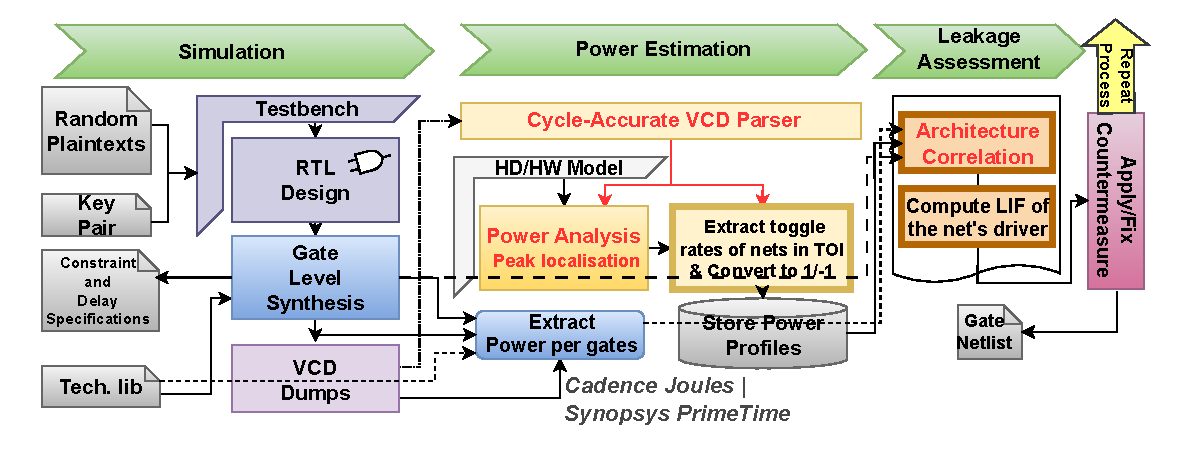
\includegraphics[width=0.5\textwidth]{Pictures/ACAnew.drawio2.pdf}
  \caption{The \methodname~methodology (this work).}
  \label{fig:ACAnew}
  \vspace{-2mm}
\end{figure}

Motivated by iterative ASIC design flow, we developed a leakage estimator that is both fast and gate-level leakage localization granularity. 
The ACA methodology namely burns \textit{days} to obtain the time-series power traces (cf.\ Table~\ref{tab:runtime_breakdown_ACA}); such long back-end runs are unacceptable during an iterative design flow. 

Our fast PSC methodology \textbf{\methodname} (\methoddis), shown in Fig.~\ref{fig:ACAnew}, retains the gate-level accuracy of ACA, yet finishes in {$<$2 h} on the same 600-trace data set for the \emph{Ibex} 
case study ({\bf a 960$\times$ speed-up}). The key idea is simple: \textit{never simulate time-series power traces}. With runtime reduced from days to a coffee break, \methodname\ provides the information needed to address vulnerabilities before the tape-out. \\


% --------------------------------------------------------------------------
\noindent{\bf Method overview. } 
Similar to the classic ACA methodology, \methodname\ also follows three phases.  We keep the \emph{Simulation} phase (RTL to gate synthesis followed by a conventional VCD dump) unchanged, and the final \emph{Leakage-assessment} phase only slightly modified. The main difference lies in the \emph{Power-estimation} phase. We employ a two-pass procedure, at the heart of which lies a cycle-accurate VCD parser: 
 the first pass is used for the peak localization, and the second pass for processing cycle-accurate VCD traces (highlighted  red in Fig.~\ref{fig:ACAnew}).\\


% --------------------------------------------------------------------------
\begin{figure}[!t]
  \centering
  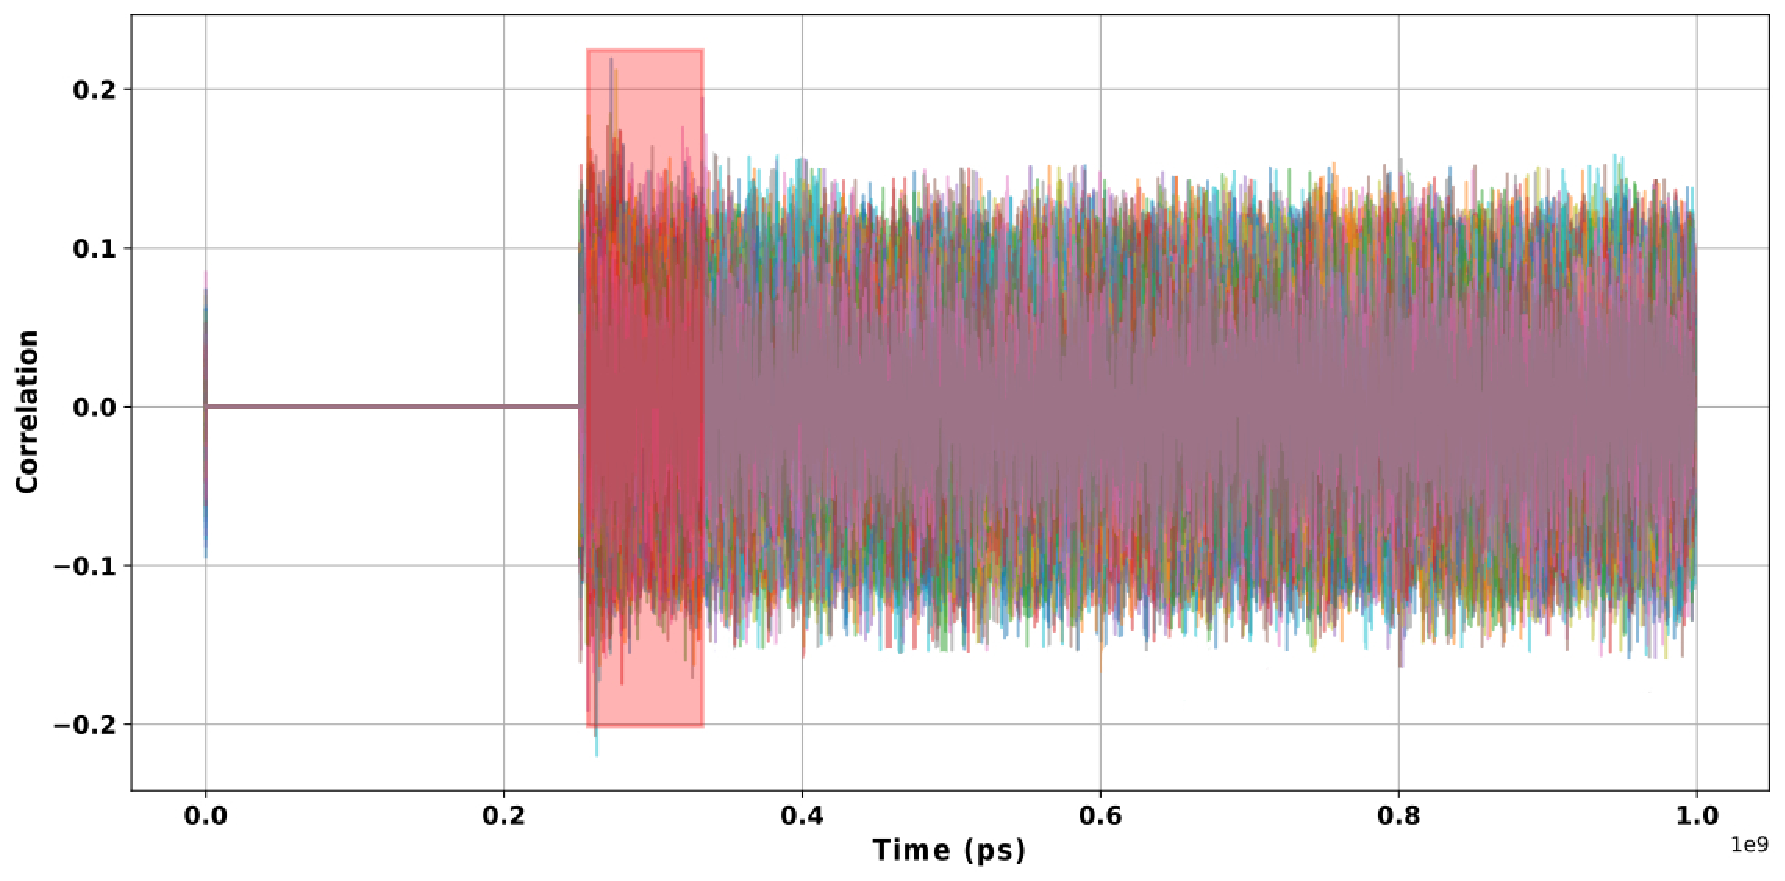
\includegraphics[width=0.9\columnwidth]{Pictures/highlighted_rectangle_fixed.pdf}
  \caption{Correlation of total toggles with 128 HD models; TOI highlighted.}
  \label{fig:Toggle_correlation}
  \vspace{-2mm}
\end{figure}

\noindent{\bf Power estimation phase - Pass 1 $\rightarrow$ Peak localization.}
In this step, we aim to identify time windows during which the design exhibits stronger leakage. Isolating such windows significantly reduces the search space and conserves computational resources. Rather than relying on precise and computationally expensive bounds, such as those used in LTI-based approaches like the classic  
      ACA flow, we look for time windows that exhibit high correlation with 
      each model in a pre-defined set of possible leakage models. 
      The results derived from this step do not directly determine the leakage model but help to limit the analysis to the most promising time regions.

To achieve this, we use the results from the Cycle-Accurate VCD Parser and calculate the total number of signal toggles across all nets at each clock edge. During peak localization we compute the Pearson correlation between the obtained toggle vector and each of the 128 HD models for Tiny-AES. The clock cycle(s) showing the highest correlation define our \emph{Time Of Interest} (TOI), as illustrated in Fig.~\ref{fig:Toggle_correlation}, where the TOI is highlighted in red. Processing the complete set of traces takes \(\approx 33\) minutes for Ibex core, This step is omitted for AES coprocessor due to its significantly smaller number of cycles.\\


% --------------------------------------------------------------------------

\noindent{\bf Robustness to the threshold. }
A practical nuisance of the classic ACA flow is the manual choice of LTI: 
shift the Pearson threshold a little and the set of
cycles classified as “leaking” changes, which may reorder the final LIF
list.  Our parser works \emph{cycle-by-cycle}: every clock edge is evaluated
individually, no binary decision “toggle inside/outside the LTI” is
required, hence the ranking is insensitive to how wide a
window the designer selects.  The benefit of a compact window such as TOI is the
runtime: a smaller slice of the data is processed, but correctness is not
affected.\\

% --------------------------------------------------------------------------

\noindent{\bf Power estimation phase - Pass 2 $\rightarrow$ Cycle-Accurate VCD Traces. }
Inside the TOI, we revisit the VCD and construct one binary toggle trace per net:
\(K_i(t) \in \{-1, +1\}\), with \(K_i(t) = +1\) if net \(i\) toggles at cycle \(t\), and \(-1\) otherwise. 
For the Ibex core, which contains approximately 8.3k nets, the parser processes each nets in about 18\,ms, resulting in a total runtime of around 2.5\,minutes for the selected time window (Tab.~\ref{tab:timing}). 
For the AES coprocessor, which includes roughly 38k nets, the total parsing time is around 2.5\,minutes, mainly due to its much smaller number of analyzed cycles.\looseness=-1

% --------------------------------------------------------------------------

\noindent{\bf Leakage assessment phase - Architecture correlation. }
For every clock cycle \(t\) we form the dot product between the leakage-model
toggle vector \(\mathbf{H}\) and the toggle vector \({K_i(t)}\) of net \(i\) obtained from the cycle-accurate VCD parser, as $C_i(t) = K_i(t) \cdot \mathbf{H}$. % shown in Eq. (\ref{eq:ACA_new}).
 A large \(C_i(t)\) means net \(i\) follows the leakage model in cycle \(t\) and is thus a likely source of leakage. Given that $K_i \in \{-1,+1\}^{j\times \mathrm{clk}}$ and $\mathbf{H}_j \in \mathbb{R}^{j\times 1}$, the results are 
$K_i\mathbf{H}_j \in \mathbb{R}^{1\times \mathrm{clk}}$ where \(j\) is the number of stimuli, \(\mathrm{clk}\) the number of clock edges, and \(i\) the total number of nets. We show this calculation in Eq. (\ref{eq:ACA_new3}). 

\begin{equation}
\mathbf{M}=\bigl[\,K_0(t)\mathbf{H}_j\; K_1(t)\mathbf{H}_j\; \dots\; K_{i-1}(t)\mathbf{H}_j\,\bigr]
\in \mathbb{R}^{i\times \mathrm{clk}},
\label{eq:ACA_new3}
\end{equation}


\begin{figure}[!t]
  \centering
  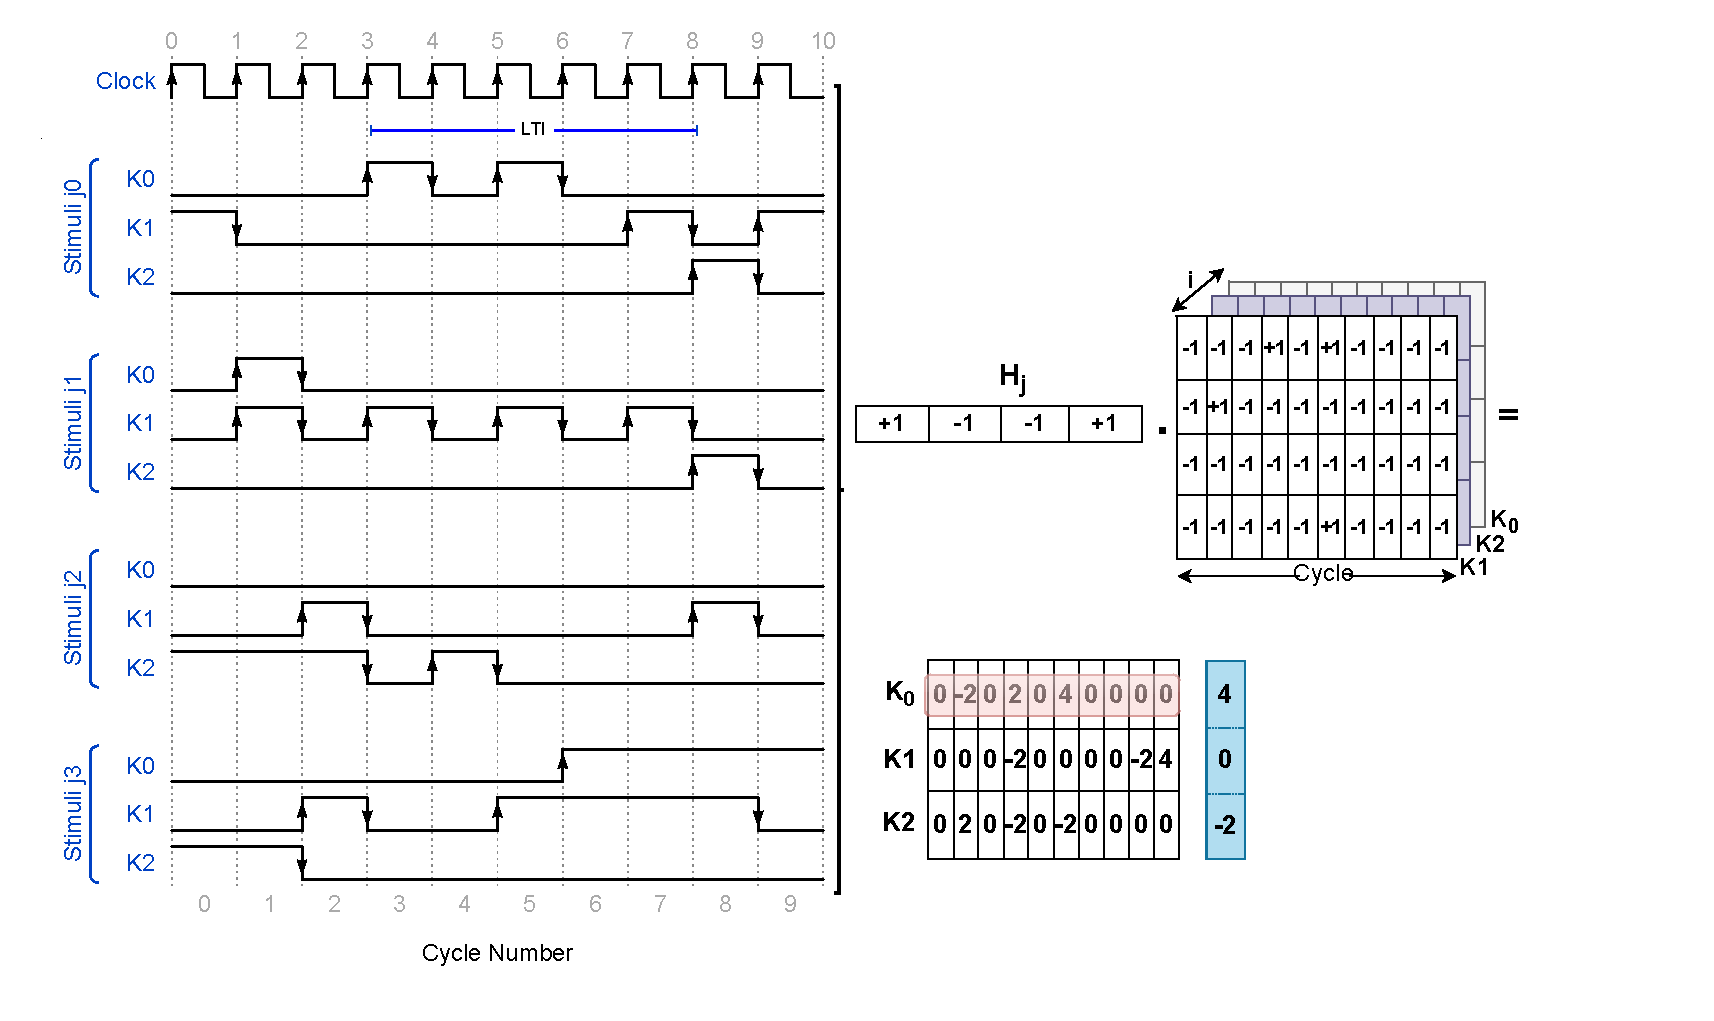
\includegraphics[width=0.53\textwidth]{Pictures/zzz_seconedition.drassswio.pdf}
  \caption{Cycle-accurate architecture correlation
           Eq. (\ref{eq:ACA_new3}) inside the TOI.  Net \(K_0\) clearly
           realizes the leakage model.}
  \label{fig:EACACAnew}
  \vspace{-2mm}
\end{figure}


Fig.~\ref{fig:EACACAnew} demonstrates an example of our methodology. The blue band highlights the LTI identified by the ACA flow method, as detailed in Table~\ref{tab:example_AC}. Whereas the time-of-interest (TOI) spans clock cycles 0–10 (all cycles in Fig. \ref{fig:EACACAnew}), the ACA flow narrows this down to cycles 3-8 (selected with blue line in Fig. \ref{fig:EACACAnew}). In that example, net (\(K_0\)) exhibits the highest architecture correlation with the leakage model \(\mathbf{H}_j\). Our approach likewise identifies net0 effectively, even without explicitly defining a precise leakage time interval beforehand. Notably, the cycle-accurate VCD parser step is executed only once, regardless of any subsequent changes to the leakage model \(\mathbf{H}_j\). i.e., the larger matrix in this example, which corresponds to the nets' activities over time \(\mathbf{K_i(t)}\), remains the same. Only the dot product with different leakage models needs to be recalculated. \\

 \begin{figure}[!t]
     \centering
     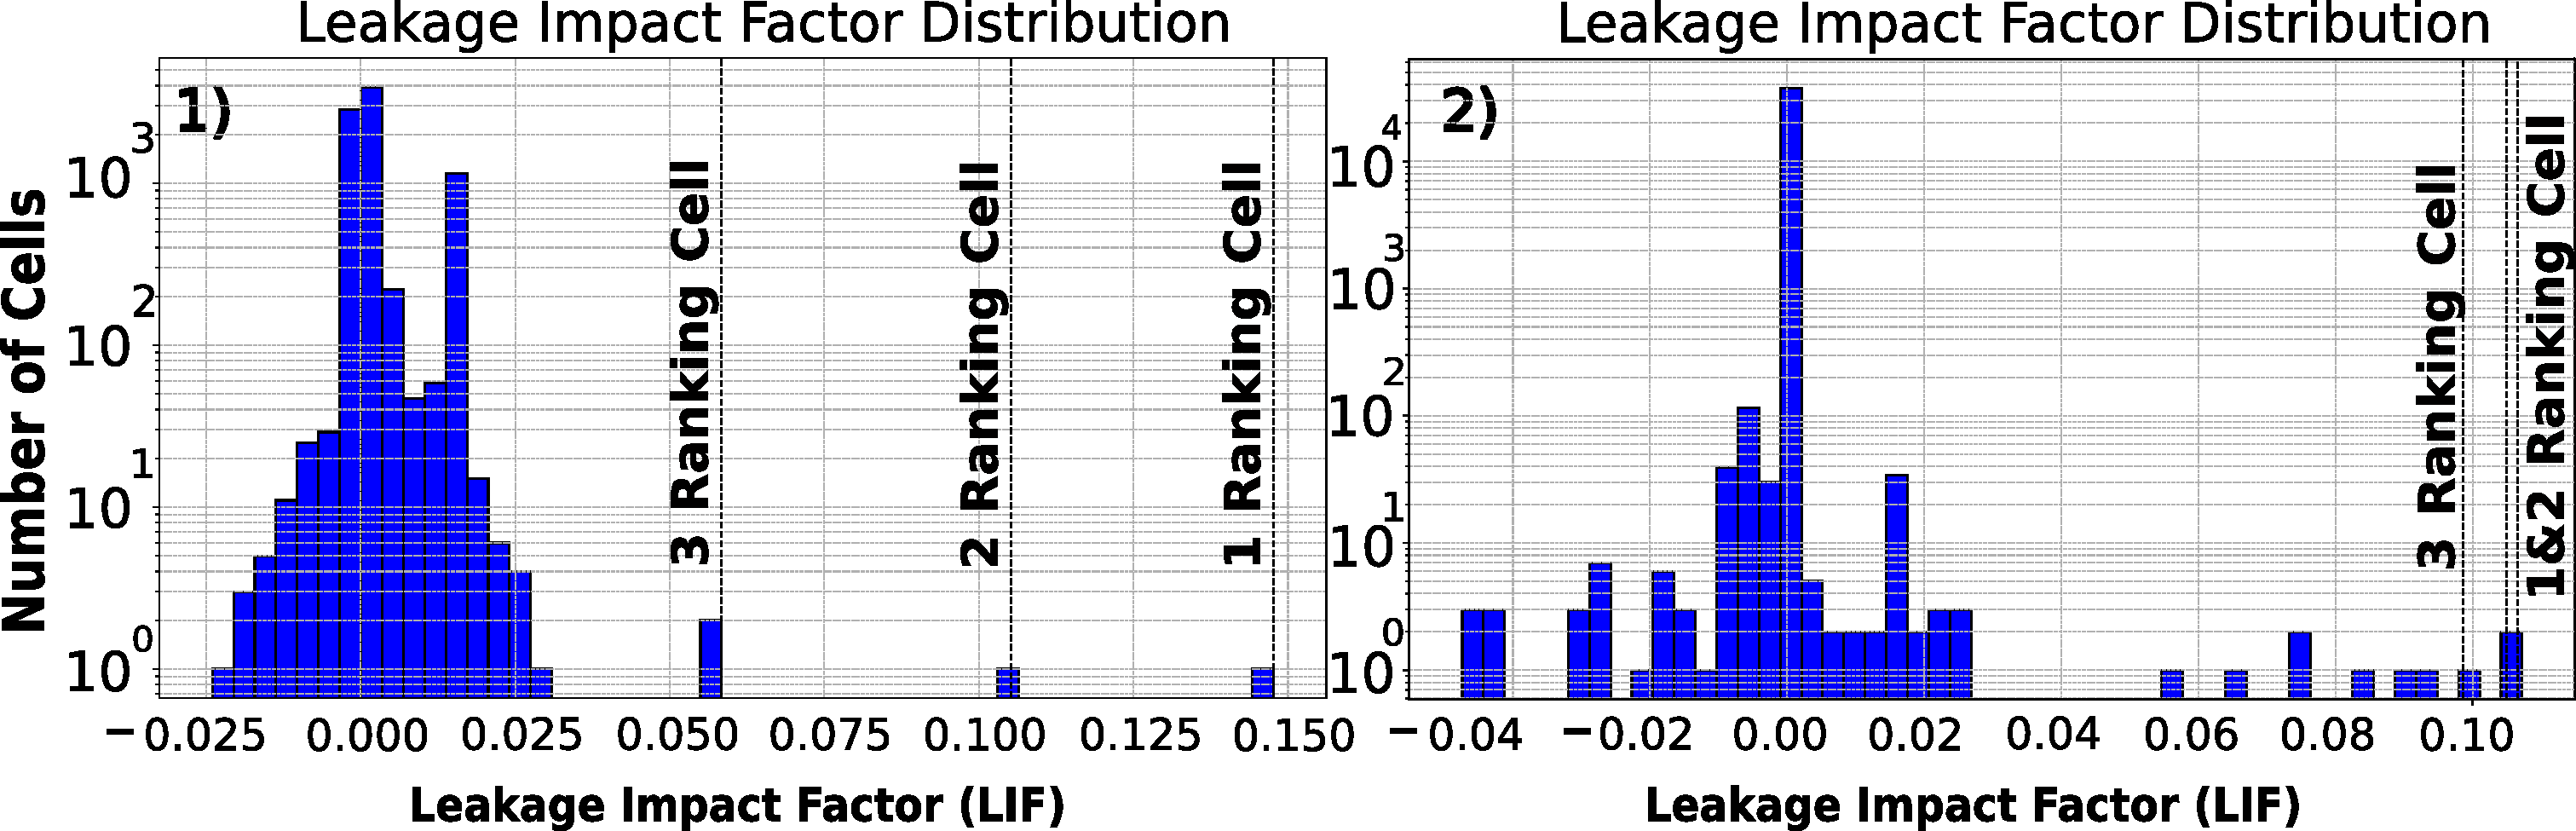
\includegraphics[width=\columnwidth]{Pictures/NETLIF_distribution_Assess_modinewbold.pdf} %vector is PDF
     \caption{{ASSESS LIF distribution for 1) 600 traces on Ibex; and 2) 1500 traces on AES coprocessor (log scale).}}
     \label{fig:newACA_LIF600}
     \vspace{-3mm}
 \end{figure}


{
\renewcommand{\arraystretch}{0.8}

\begin{table*}[t]
\centering
\setlength{\tabcolsep}{8pt}
\caption{\methodname{} end-to-end runtime on Ibex and on the AES coprocessor.}
\label{tab:timing}

\begin{tabular}{l|p{0.37\textwidth}cccc}%\begin{tabularx}{\textwidth}{l|Xcccc}
\hline
\multicolumn{2}{c}{} &
\multicolumn{2}{c}{\textbf{Ibex (600 traces)}} &
\multicolumn{2}{c}{\textbf{AES coprocessor (1500 traces)}} \\
\cline{3-6}
\textbf{Phases} & \textbf{Step} &
\textbf{Per-trace} & \textbf{Total} &
\textbf{Per-trace} & \textbf{Total} \\ \hline

\multirow{3}{*}{Sim.}
& Vmem gen.\ (shared)     & 141\,ms    & 1\,m\,24\,s  & —          & — \\
{}
& Synthesis (once)        & —          & 5\,m\,53\,s  & —          & 36\,m\,9\,s \\
{}
& VCD dump                & 6.3\,s     & 1\,h\,3\,m   & 3\,s       & 1\,h\,15\,m \\ \hline

\multirow{4}{*}{Pwr.\ Est.}
& \emph{Step 1: Peak localisation}
                          & 3.3\,s     & 33\,m\,6\,s  & —          & — \\
{}
& \emph{Step 2: Cycle-accurate VCD parser}
                          & 56.4\,it/s & 2\,m\,28\,s  & 10.4\,it/s & 2\,m\,24\,s \\
{}
& Per-gate power scan     & —          & 19\,s        & —          & 2\,m\,49\,s \\
{}
& Calculate $C_i$         & —          & 3\,m\,31\,s  & 480\,it/s  & 1\,m\,18\,s \\ \hline

Lkg.A.
& Net-list parsing \& LIF  & 40\,nets/s & 3\,m\,28\,s  & 12.5\,nets/s & 50\,m\,12\,s \\ \hline

\multicolumn{2}{l}{end-to-end runtime}
&  & \textbf{1\,h\,53\,m\,9\,s}
&  & \textbf{$\approx$\,2\,h\,42\,m} \\ \hline
\end{tabular}%\end{tabularx}
\end{table*}

}

\noindent{\bf Leakage assessment phase - LIF estimation. }
For each net \(i\), the parser yields a toggle vector; dot products with
the HD leakage model produce the architectural correlation \(C_i\).
Multiplying \(C_i\) by the normalized average gate power
\(P_i/P_T\) yields the LIF, consistent with the ACA flow.
The histograms in Fig.~\ref{fig:newACA_LIF600} exhibit the typical long-tail shape:
in both designs, a single flip-flop dominates the leakage. 
For the Ibex core, the top-ranked element is a flip-flop within the register file that stores the 128-bit AES state,
whereas in the AES coprocessor it is a flip-flop within the 128-bit state register itself.
All remaining gates (over 8K nets in Ibex and 37K nets in the AES coprocessor) contribute only marginally.





\noindent{\bf Timing results (concise).}
Processing \(600\) traces on Ibex core completes in \textbf{1\,h\,53\,min} (Table~\ref{tab:timing}).  
A one-off \emph{pre-processing} phase (VMEM generation + gate-level synthesis) accounts for only \(\approx 6\%\) (\(\sim7\) min) of the end-to-end runtime.  
The VCD dump dominates at \(\approx56\%\), peak localisation adds \(\approx29\%\), and all remaining steps together contribute the final \(\approx9\%\).  
Overall, the flow achieves a speed-up of \(\mathbf{960\times}\) over classical ACA and \(\mathbf{1{,}030\times}\) over PATCH on the same Ibex benchmark. \\
Processing the {AES coprocessor} design (\(1{,}500\) traces) completes in \textbf{2\,h\,42\,min}.  
Although the design is approximately \(4.7\times\) larger than Ibex, its shorter 11-cycle operation substantially reduces the time required for generating power traces.  
About \(46\%\) of the total runtime is spent on VCD dumping, while parallelism and the lower cycle count make the VCD parsing phase faster, consuming only \(\sim2\%\) of the total time.  
Netlist parsing and LIF estimation remain the most time-intensive software phase (\(\sim31\%\)), primarily due to the higher gate count.  
It is also notable that, owing to this larger design, the per-gate power scan with CPT (Joules) takes slightly longer than in Ibex, yet still accounts for only about \(2\%\) of the total runtime.  
Overall, our method achieves a \textbf{3.8$\times$} speed-up compared to the ACA flow on this design. \\

{
\renewcommand{\arraystretch}{0.9} % shrink row height just inside this group

\begin{table*}[!]
\centering
\caption{Comparison of pre-silicon PSC leakage evaluation methodologies.}
\label{tab:comparison}
\small
\setlength{\tabcolsep}{3pt}  % slightly tighter columns

% l = first label column
% X = flexible-width description column (can wrap)
% c c c c = four method columns
\begin{tabular}{l p{0.33\textwidth} c c c c}%\begin{tabularx}{\textwidth}{l X c c c c}
\hline
 &  & \textbf{ASSESS (this work)} & \textbf{ACA~\cite{ACA}} &
       \textbf{PATCH~\cite{PATCH}} & \textbf{RTL-PAT~\cite{RTL_PSC}} \\
\hline
Design stage              &                                  & Gate level      & Gate level      & Gate level      & RTL \\
Technology dependency     &                                  & Yes             & Yes             & Yes             & No \\
CPT dependency            &                                  & Yes             & Yes             & Yes             & No \\
Localization granularity  &                                  & Fine (net/gate) & Fine (net/gate) & Medium (net)    & Coarse (module) \\
Toggle                    &                                  & \ding{52}       & \ding{52}       & \ding{52}       & \ding{52} \\
Delay-aware               &                                  & \ding{52}       & \ding{52}       & \ding{52}       & \ding{55} \\
Sample rate               &                                  & 2               & user defined    & user defined    & 2 \\
\hline
\multirow{2}{*}{Advantage}
  & Leakage assessment at gate level                       & \ding{52} & \ding{52} & \ding{52} & \ding{55} \\
  & LIF per gate                                           & \ding{52} & \ding{52} & \ding{55} & \ding{55} \\
\hline
\multirow{2}{*}{Drawback}
  & Data collection cost                                   & Low       & High      & High      & Medium \\
  & Probability of undiscovered leakage sources            & Low       & Low       & Medium    & High \\
\hline
\multirow{2}{*}{end-to-end$^{\mathrm{*}}$ runtime}
  & data collection                                        & $\approx 1$ hour & $>72$ days & $>72$ days & $\approx 1$ hour \\
  & analysis                                               & $<1$ hour        & $>2$ hours & $>6$ hours & $<1$ hour \\
\hline
\multicolumn{6}{l}{$^{\mathrm{*}}$ Data from Tables~\ref{tab:pscrtl_timing}, \ref{tab:patchruntime_breakdown}, \ref{tab:runtime_breakdown_ACA}, and \ref{tab:timing}.}
\\\hline
\end{tabular}%end{tabularx}
\vspace{-1mm}
\end{table*}
}
\noindent{\bf Runtime comparison and methodology summary.}
In Table~\ref{tab:comparison} we provide a summary of the systematic comparison of three state-of-the-art pre-silicon PSC leakage evaluation methodologies RTL-PAT, PATCH, and ACA, and compare them with the proposed methodology \methodname. We then list the advantages and drawbacks of each methodology and summarize their runtimes based on our experiments. Like all gate-level methodologies, \methodname\ remains dependent on a technology-specific standard-gate library and at least one commercial power estimation run to obtain the LIFs. Data collection cost and runtime for \methodname{} are much lower, primarily due to the reduced reliance on time-series power trace. The sampling rate reported in Table~\ref{tab:timing} is used only for identifying the TOI during peak localization. Once the TOI is determined, the leakage assessment itself is performed using cycle-accurate switching activity, which follows the same mathematical principle as the correlation used in ACA. Since our methodology intentionally considers a broader time window rather than narrowly defined leakage intervals, the risk of missing relevant leakage activity is reduced.




Pre-silicon runtime depends primarily on the number of simulated samples (\textit{latency} $\times$ \textit{samples/cycle}) and tool/node settings rather than netlist size alone.  
As Table~\ref{tab:runtime_context} shows, ACA’s 11-cycle AES coprocessor costs \(\approx18\) s per trace, whereas our Ibex running Tiny-AES executes \(\approx10{,}000\) cycles and thus \(\approx2\,\mathrm{h}\,54\,\mathrm{m}\) per trace—consistent with this dependency, the total column indicates the approximate time required to collect 600 traces.
RTL-PAT~\cite{RTL_PSC}, with \(>\!3\)k cycles, reports an end-to-end runtime of \(\approx30\) h.  
Fig.~\ref{fig:AESDesign_CO_LTI} further illustrates this trend: the projected speed-up increases with both design size and the number of simulated cycles.  
In regions where these factors are high, the proposed method provides the greatest advantage, as power-trace extraction becomes the dominant bottleneck in traditional ACA-style flows.


The cycle-accurate, VCD-driven, gate-level \methodname\ methodology achieves the 
\emph{fine localization granularity} of the classical ACA approach. 
% \emph{same localization granularity} as the classical ACA approach. 
By parsing toggles once and avoiding repeated CPT trace simulators, \methodname\ reduces the end-to-end runtime on Ibex RISC-V core from \textbf{72 days to \(\approx1\) h}.  
It is roughly \(10^{3}\!\times\) faster than PATCH and delivers a further \(9\%\) improvement over RTL-PAT while offering much finer localization granularity.  
During analysis, each net’s toggles are captured at every clock edge after delay annotation.
\section{Conclusions}
\label{sec:Conclusions}

\begin{figure}[!t]
  \centering
  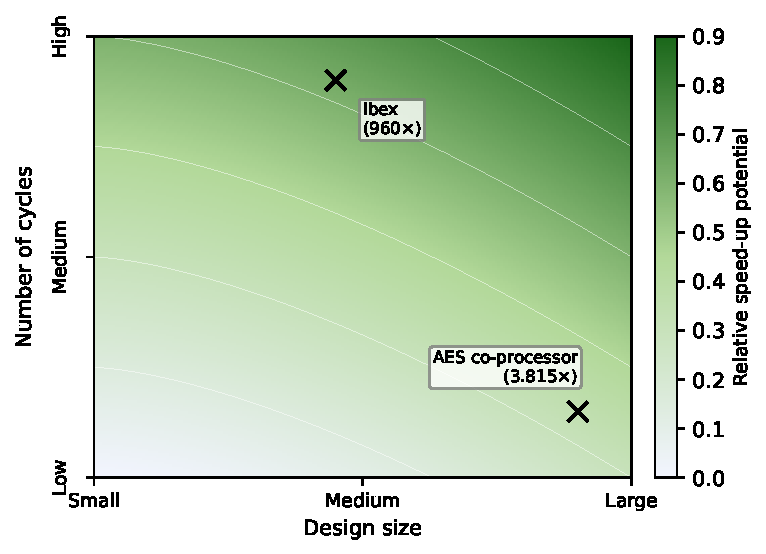
\includegraphics[width=0.84\columnwidth]{Pictures/Conceptual_relation.pdf}
  \caption{\methodname{} speed-up potential.}
  \label{fig:AESDesign_CO_LTI}
  \vspace{-3mm}
\end{figure}
This paper presented a thorough qualitative and quantitative comparison of three prominent pre-silicon power side-channel analysis methodologies, namely RTL-PAT, PATCH, and ACA, and introduced an enhanced ACA-inspired methodology called \methodname{}. Our experiments, performed on a RISC-V CPU core running Tiny-AES at the 22nm technology node, revealed the following.  RTL-PAT is fast and can be applied early in the design cycle, but lacks gate-level localization. PATCH and ACA offer more fine-grained leakage localization,
%insights into leaky signals or gates; 
however, both incur considerable runtime overhead due to extensive time-series power extraction.
\methodname{} is a cycle-accurate, VCD-driven methodology operating at the gate-level abstraction. It retains ACA’s fine-grained localization ability while avoiding its most time-consuming steps. Our experimental results validate that \methodname\ substantially accelerates analysis without sacrificing accuracy, making it better suited for iterative ASIC design cycles  %processes 
in advanced technology nodes. By open-sourcing all implementations, we aim to establish a common baseline for future improvements in pre-silicon PSC leakage evaluations. Ultimately, our work highlights the importance of robust pre-silicon PSC leakage evaluations and provides a practical methodology for designing secure hardware in modern ASIC design flows.

{

\begin{table}[h]
\centering
%\footnotesize
\caption{Complexity of benchmarks \& CPT runtimes}
\label{tab:runtime_context}

\begin{tabular}{lcccc}
\hline
 & \multicolumn{2}{c}{Benchmark} & \multicolumn{2}{c}{CPT Runtime} \\
\cline{2-5}
 & \# gates & \# cycles & per trace & total \\
\hline
AES coprocessor~\cite{projectvault_aes_verilog}
 & $\approx$38k & 11 & $\approx$18\,s & $\approx$3\,h \\

SoC bus~\cite{ACA}
 & 100k & $\approx$26 (LTI) & $\approx$329\,s & $\approx$60\,h \\

Ibex (this work)
 & $\approx$8k & $\approx$10k & 2\,h\,54\,m & $\approx$70\,d \\
\hline
\end{tabular}
\vspace{-3mm}
\end{table}
}

\begin{acks}
This work was funded by the Dutch Research Council (NWO) through the PROACT project~\cite{PROACT} (NWA.1215.18.014).
\end{acks}






\bibliographystyle{ACM-Reference-Format}
\bibliography{ACM2/bilbio}

\end{document}
